%=======================================================
%	PACKAGES AND THEMES
%=======================================================
\documentclass[8pt]{beamer}
\mode<presentation> {
\usepackage{etex}
\usetheme{Boadilla}
\definecolor{navyblue}{rgb}{0.0, 0.0, 0.5}
\definecolor{dkgreen}{rgb}{0,0.6,0}
\definecolor{gray}{RGB}{64, 64, 64}
\definecolor{mauve}{rgb}{0.58,0,0.82}
\usecolortheme[named = navyblue]{structure}
\setbeamercolor{normal text}{fg = gray}
\setbeamercolor{frametitle}{fg = white, bg = navyblue}
\setbeamerfont{framesubtitle}{size = \normalsize}
\setbeamerfont{caption}{size=\footnotesize}
\setbeamercolor{page number in head/foot}{fg = gray}
\setbeamertemplate{footline}%[frame number]
}


\usepackage{graphicx} % Allows including images
\usepackage{booktabs} % Allows the use of \toprule, \midrule and \bottomrule in tables
\usepackage{multicol}
\usepackage[export]{adjustbox}
\usepackage{colortbl}
\usepackage{graphicx} 

\usepackage{tikz}
\usepackage{fancybox}
\usepackage[absolute, overlay]{textpos}
\usepackage{multirow}
\usepackage{siunitx}
\usepackage{tcolorbox}


\usepackage{tikz}
\usepackage{calc}
\newlength{\outerradius}
\newlength{\innerradius}
\setlength{\outerradius}{0.50cm}
\setlength{\innerradius}{0.35cm}

%Damit wir Quellcode nutzen können.
\usepackage{listings}
\lstset{numbers=left,
	numberstyle=\tiny,
	numbersep=5pt,
	breaklines=true,
	showstringspaces=false,
	frame=l ,
	xleftmargin=15pt,
	xrightmargin=15pt,
	basicstyle=\ttfamily\scriptsize,
	stepnumber=1,
	keywordstyle=\color{blue},          % keyword style
  	commentstyle=\color{dkgreen},       % comment style
  	stringstyle=\color{mauve}         % string literal style
}
%Sprache Festelegen
\lstset{language=R}


%=======================================================
%	TITLE PAGE
%=======================================================

\title{\textbf{Principles of Infographics}}

\author{Dr Daniele Rotolo}

\institute
{
SPRU (Science Policy Research Unit) \\
Business School\\
University of Sussex \\

\medskip

\medskip

\medskip

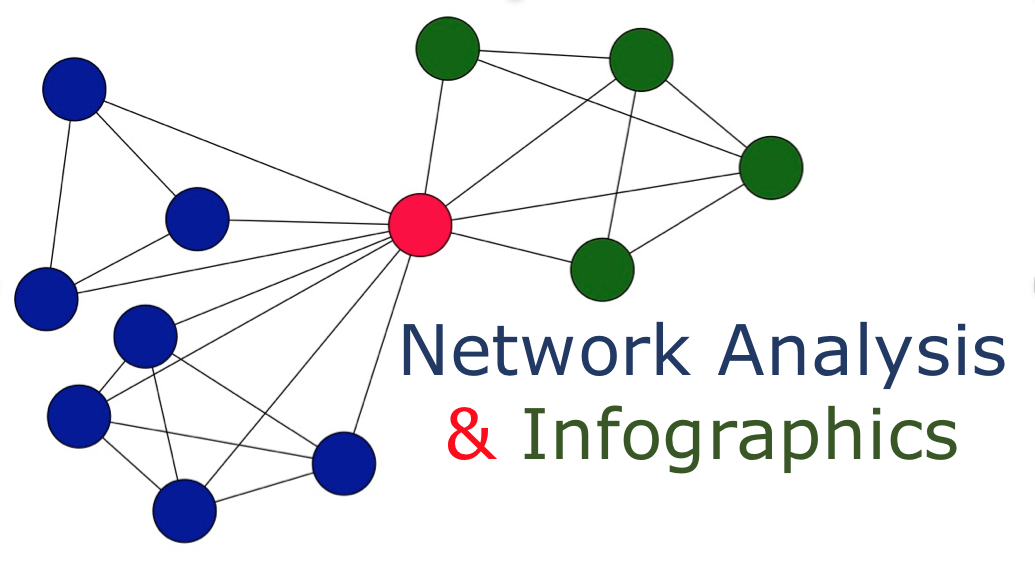
\includegraphics[width=2.5cm]{../_shared_pics/logo}

\medskip

\textit{{\color{dkgreen}{Week 7}}}\\
}


\date{} % Date, can be changed to a custom date

\begin{document}

\begin{frame}
\titlepage % Print the title page as the first slide

\begin{textblock*}{10pt}(0pt, 0.9\textheight)

\includegraphics[width=4cm]{../_shared_pics/SPRU.png}
\end{textblock*}

\end{frame}


%=======================================================
%	Learning outcomes
%=======================================================

\begin{frame}
\frametitle{Learning Outcomes}

\centering
\footnotesize
\begin{tabular}{lp{5.5cm}l}
\toprule
\multicolumn{2}{l}{\textbf{Learning outcome}} & \textbf{Assessment mode}\\
\hline
\\
1 & 
Explain the concept of network and list the main network indicators & 
ESS\\
\\
2 & 
Describe and apply the major techniques for the collection of network data and their statistical analysis & 
ESS, GPN + GWS\\
\\
3 & 
Identify the main characteristics of networks by means of network measures  & 
ESS, GPN + GWS\\
\\
\rowcolor{green!20}4 &
Employ network analysis techniques to produce network data-based infographics & 
GPN + GWS\\
\\
\bottomrule
\multicolumn{3}{l}{Note: ESS: Essay; GPN: Group Presentation; GWS: Group Written Submission}\\
\end{tabular}

\end{frame}

%------------------------------------------------






%=======================================================
% Intro slides
%=======================================================
\section*{Overview}
%------------------------------------------------

\begin{frame}
\frametitle{\insertsection}
\tableofcontents[hideallsubsections]
\end{frame}





%=======================================================
% Why infographics?
%=======================================================
\section{Why infographics?}
%------------------------------------------------

\bgroup
\setbeamercolor{background canvas}{bg = navyblue}
\begin{frame}[plain]{}
\begin{center}
\color{white}{\Huge\insertsection}
\end{center}
\end{frame}
\egroup

%------------------------------------------------

\begin{frame}
\frametitle{\insertsection}

\begin{columns}[c]
\column{.45\textwidth} 
    \begin{itemize}
    \item Half of our brain is dedicated to {\color{blue}{processing visual signals}} (we can process images {\color{blue}{60,000 times faster}} than text)
    \item Increasing capabilities to {\color{blue}{collect}}, {\color{blue}{store}} and {\color{blue}{analyse}} data (e.g.\ government data, APIs, Big Data, Data Science)
    \item Risk of information {\color{red}{overload}}
\end{itemize}

\column{.45\textwidth}
\centering
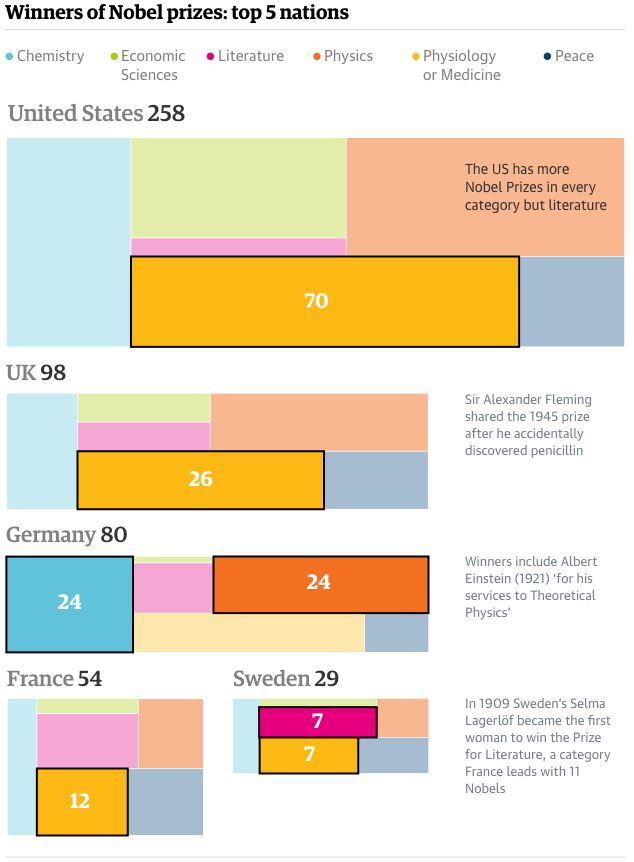
\includegraphics[width=\linewidth]{nobel}\\
\tiny{Source: \href{www.theguardian.com/science/datablog/2016/oct/08/which-countries-have-had-the-most-nobel-prize-winners}{The Guardian} (October, 2016)}

\end{columns}

\end{frame}

%------------------------------------------------

\begin{frame}
\frametitle{\insertsection}
\centering
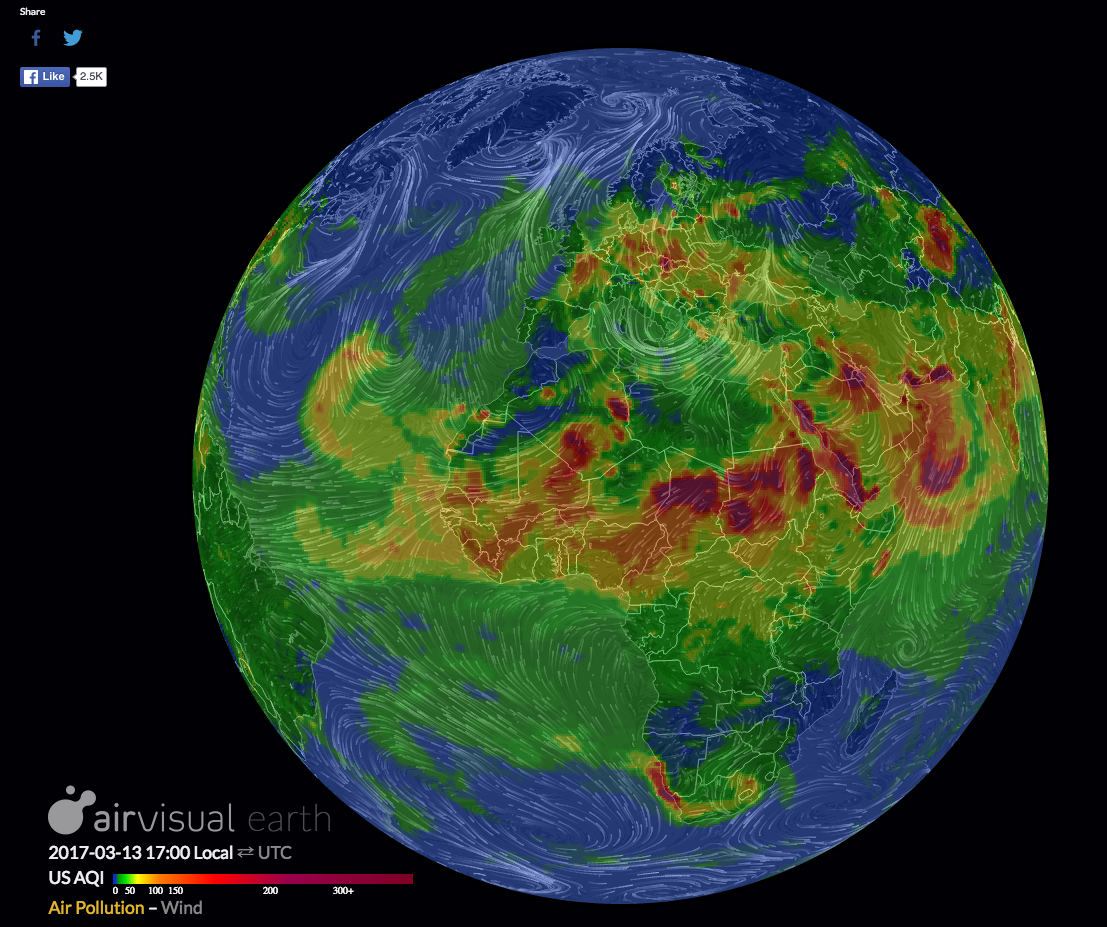
\includegraphics[width=0.75\linewidth]{airpoll}\\
\tiny{Source: Air pollution (March, 2017) [\url{https://airvisual.com/earth}]}
\end{frame}

%------------------------------------------------

%\begin{frame}
%\frametitle{\insertsection}
%\centering
%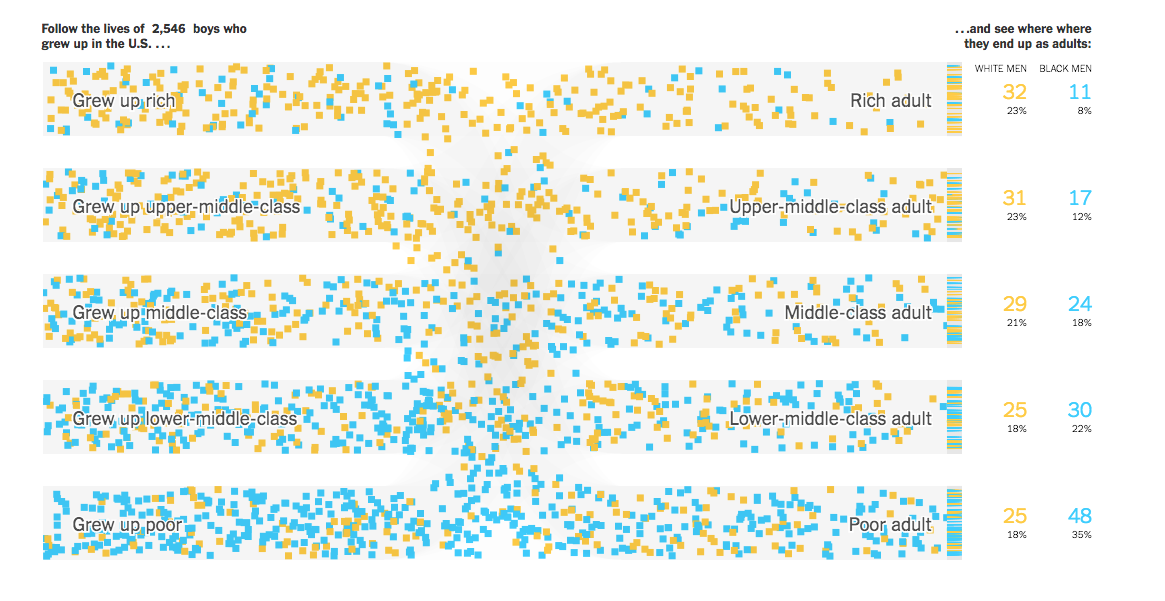
\includegraphics[width=0.9\linewidth]{racism}\\
%\tiny{Source: Punishing reach of racism [\url{www.nytimes.com/interactive/2018/03/19/upshot/race-class-white-and-black-men.html}]}
%\end{frame}
%
%%------------------------------------------------

\begin{frame}
\frametitle{\insertsection}
\centering
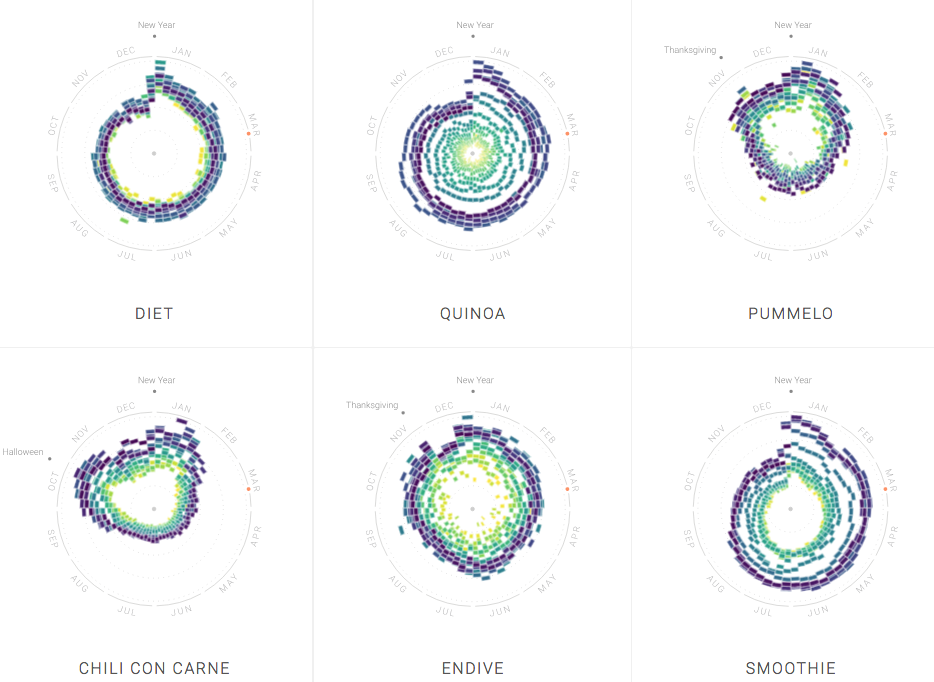
\includegraphics[width=0.9\linewidth]{food}\\
\tiny{Source: Rhythm of food [\url{http://rhythm-of-food.net}]}
\end{frame}

%------------------------------------------------

\begin{frame}
\frametitle{\insertsection}
\centering
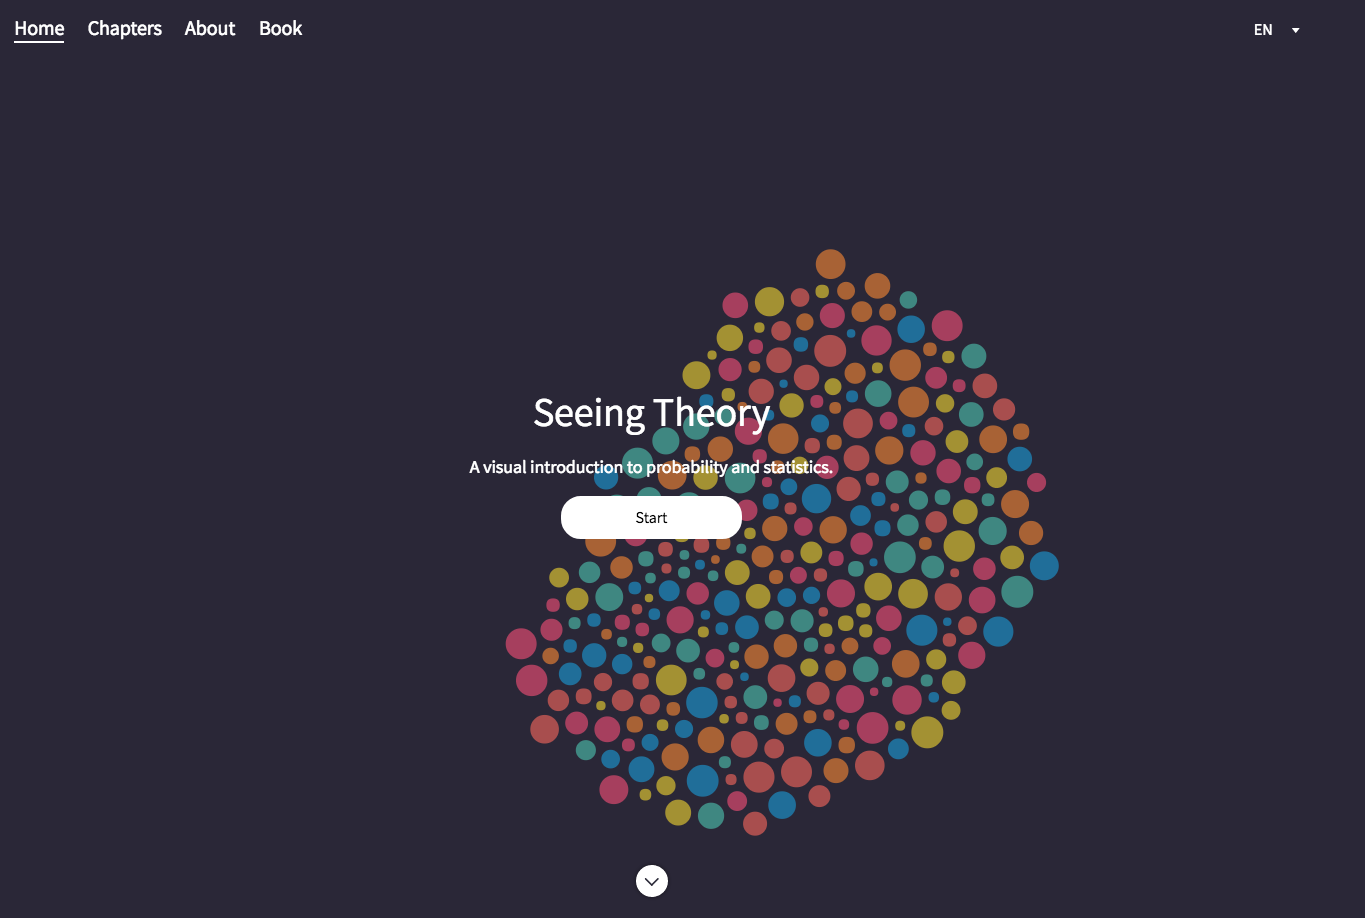
\includegraphics[width=0.9\linewidth]{seeing_theory}\\
\tiny{Source: Seeing theory [\url{http://students.brown.edu/seeing-theory}]}
\end{frame}

%------------------------------------------------

\begin{frame}
\frametitle{\insertsection}
\centering
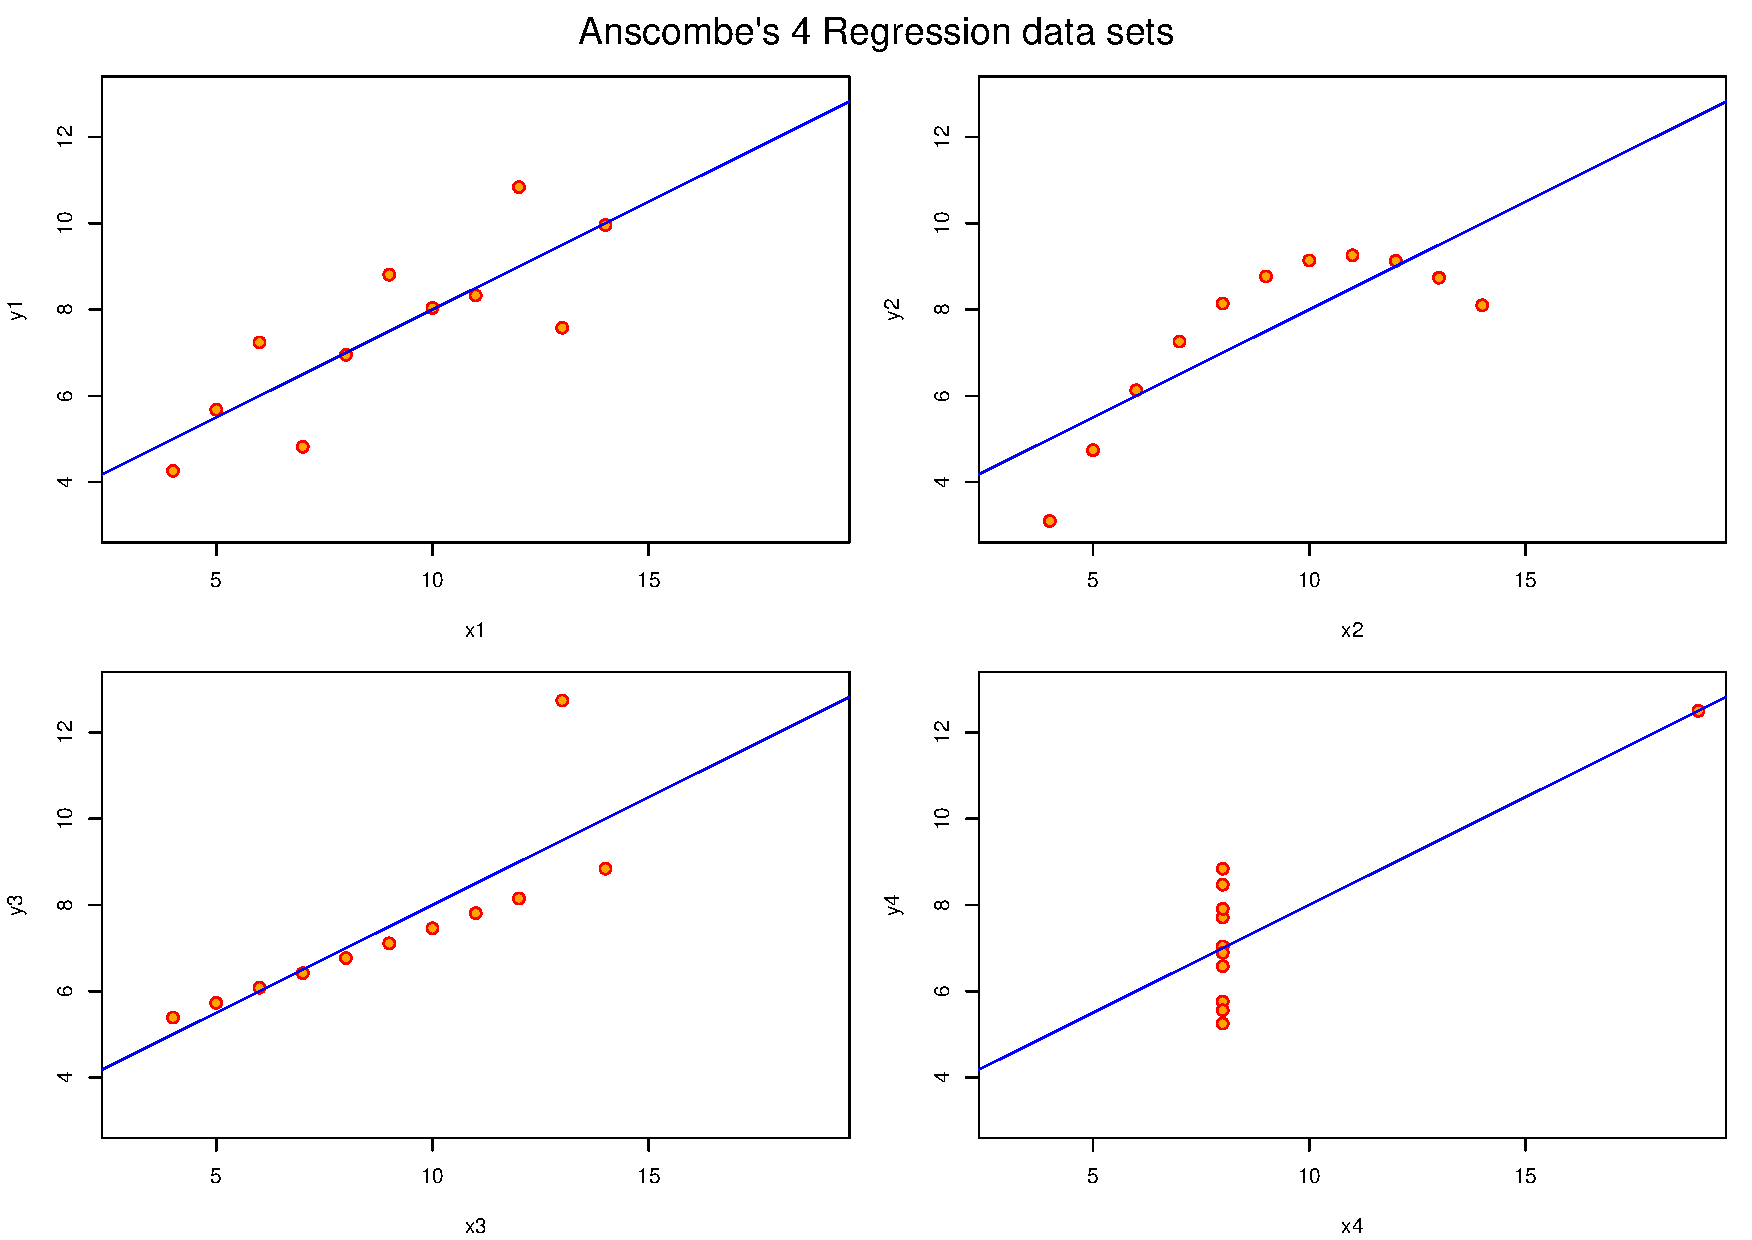
\includegraphics[width=0.9\linewidth]{anscombe}\\
\end{frame}

%------------------------------------------------

\begin{frame}
\frametitle{\insertsection}

\begin{columns}[c]
\column{.45\textwidth} 
    \begin{itemize}
    \item {\color{blue}{Raw data}} do not tell as much
    \item {\color{blue}{Statistics}} and {\color{blue}{visualisation}} help us to go beyond raw data (patterns, relationships)
    \item Infographics helps us to tell a {\color{blue}{story}}, to trigger {\color{blue}{emotions}} and {\color{blue}{actions}}
\end{itemize}

\column{.45\textwidth}
\centering
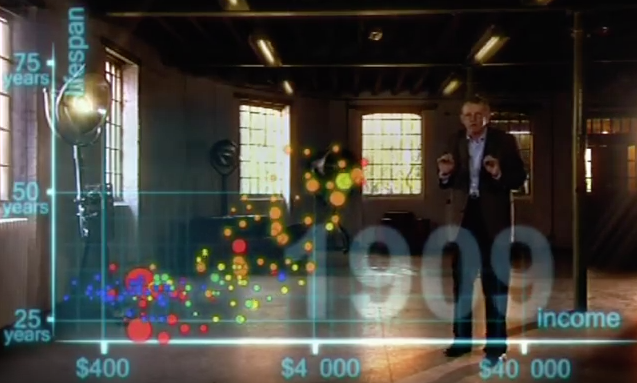
\includegraphics[width=5cm]{gapminder}\\
\tiny{Source: Hans Rosling's 200 Countries, 200 Years (\url{www.youtube.com/watch?v=jbkSRLYSojo})}
\end{columns}

\end{frame}

%------------------------------------------------




%=======================================================
% Designing infographics
%=======================================================
\section{Designing infographics}

%------------------------------------------------

\begin{frame}
\frametitle{\insertsection}

Check-list when producing an infographic
\begin{itemize}
\item Use {\color{blue}{appropriate charts}} to visualise your data
\item Explain {\color{blue}{encoding}} (e.g.\ legend)
\item {\color{blue}{Label}} axis
\item Include {\color{blue}{sources}} (e.g.\ figures, data)
\item Maximise the {\color{blue}{data-ink ratio}}
\item Ensure {\color{blue}{graphical integrity}}
\end{itemize}

\end{frame}

%------------------------------------------------

\begin{frame}
\frametitle{\insertsection}
\framesubtitle{Use appropriate charts}

\centering
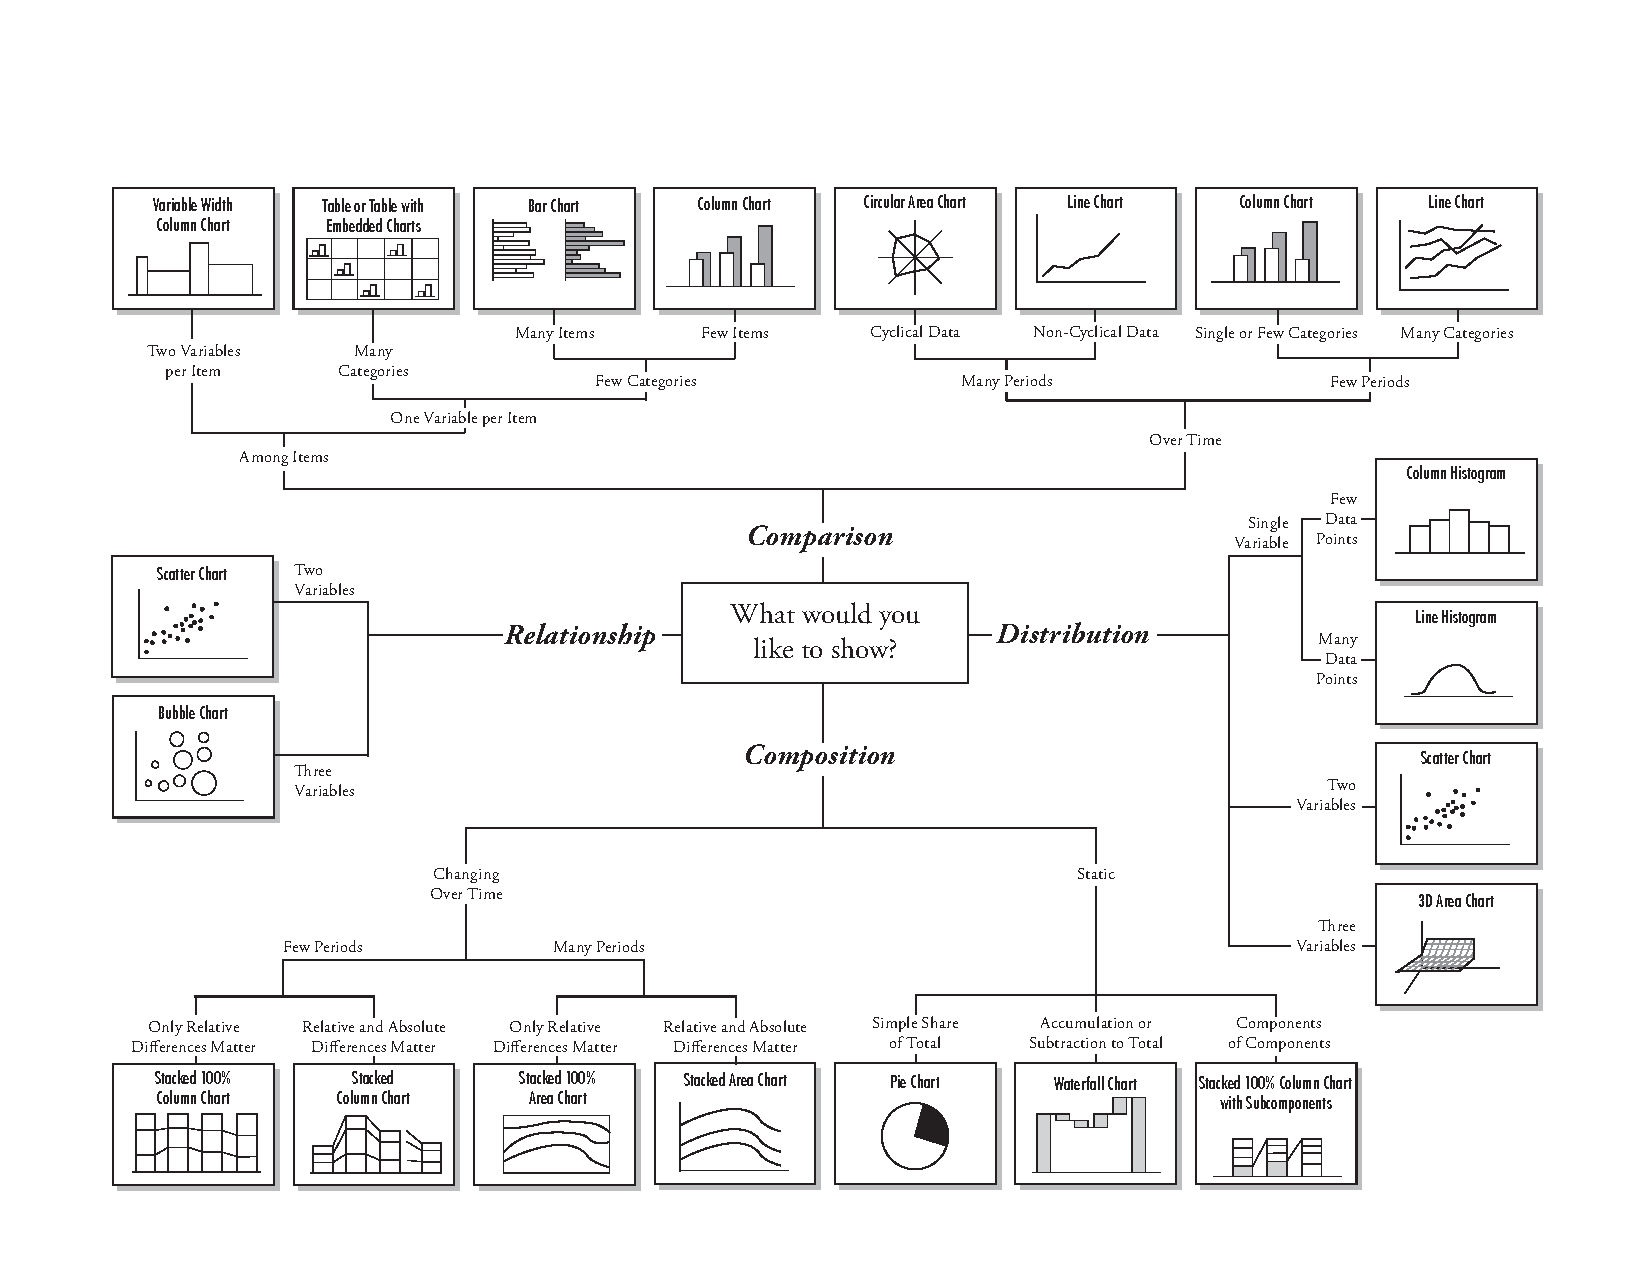
\includegraphics[width=0.85\linewidth]{chart_selection}\\
\tiny{Source: Andrew Abela [\url{https://extremepresentation.com/}]}

\end{frame}

%------------------------------------------------

\begin{frame}
\frametitle{\insertsection}
\framesubtitle{Explain encoding}

\begin{columns}[t]
\column{.5\textwidth}
\centering
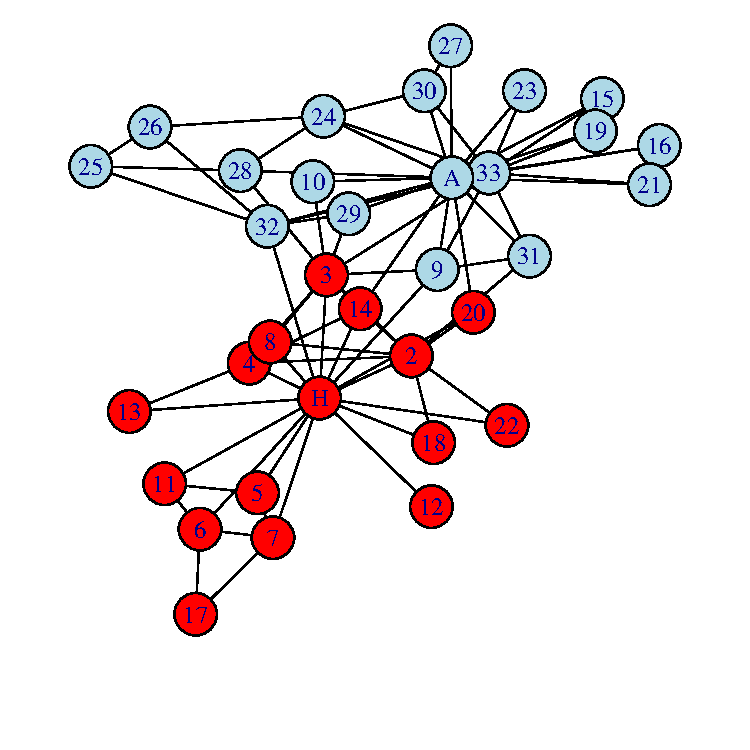
\includegraphics[width=0.9\linewidth]{karate_nl}\\
\tiny Source: Karate club network (igraphdata) \cite{Zachary1977}


\column{.5\textwidth}
\centering
\onslide<2>{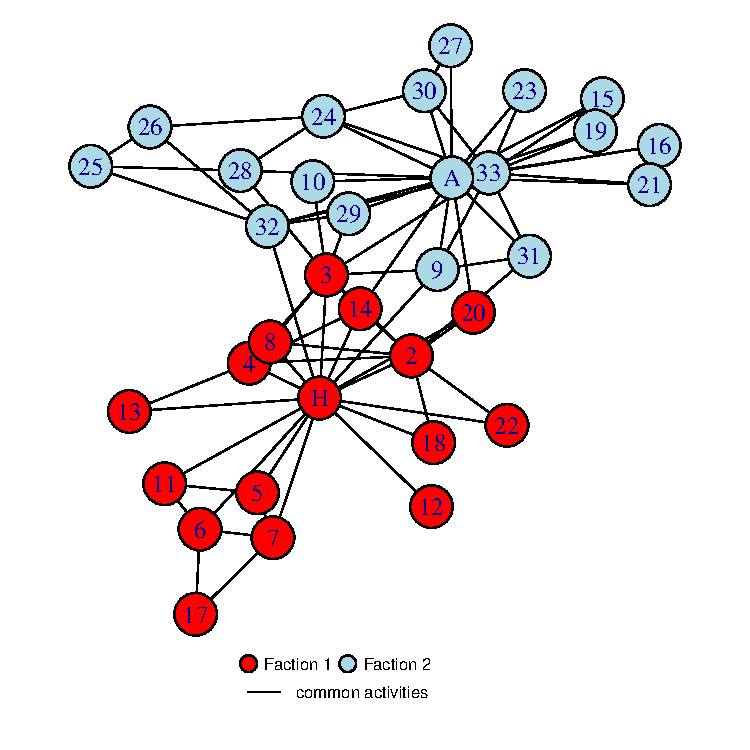
\includegraphics[width=0.9\linewidth]{karate_l}\\
\tiny Source: Karate club network (igraphdata) \cite{Zachary1977}}

\end{columns}

\end{frame}

%------------------------------------------------

\begin{frame}
\frametitle{\insertsection}
\framesubtitle{Label axis}

\begin{columns}
\column{.5\textwidth}
\centering
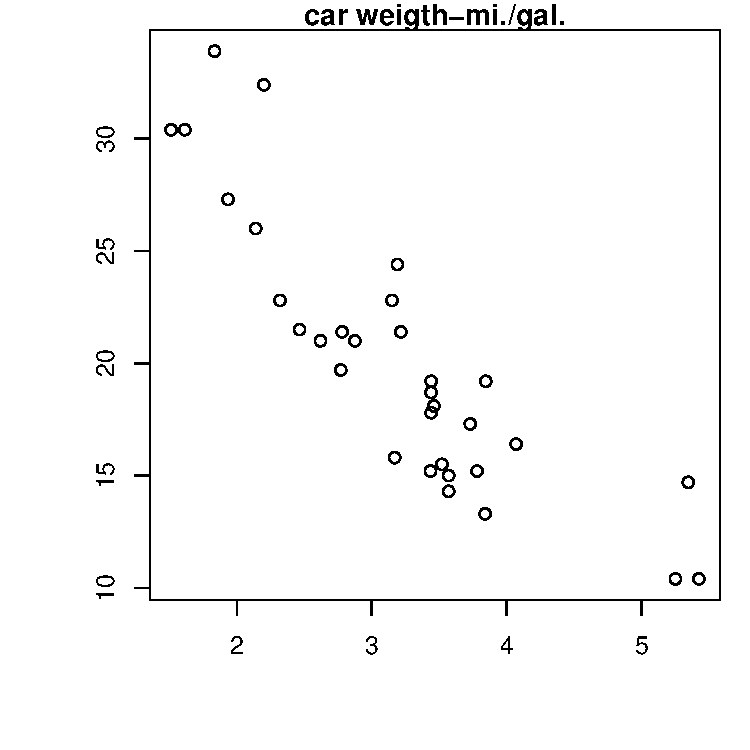
\includegraphics[width=0.9\linewidth]{label_axis_nl}


\column{.5\textwidth}
\centering
\onslide<2>{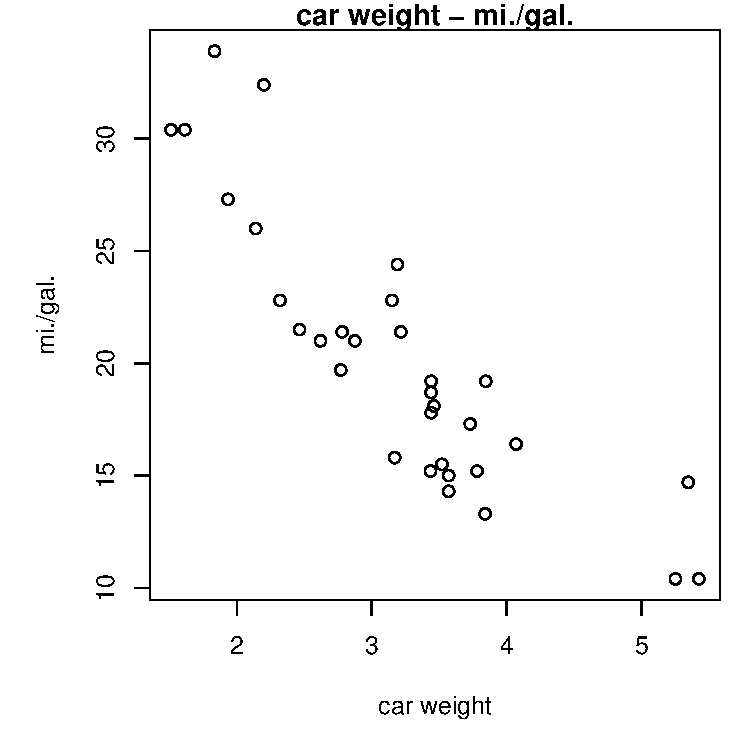
\includegraphics[width=0.9\linewidth]{label_axis_l}}

\end{columns}

\end{frame}

%------------------------------------------------

\begin{frame}
\frametitle{\insertsection}
\framesubtitle{Include sources}

\begin{itemize}
\item Recognise others' work (IPR)
\item Risk of {\color{red}{plagiarism}}
\item Text, images, and data
\end{itemize}


\end{frame}

%------------------------------------------------

\begin{frame}
\frametitle{\insertsection}
\framesubtitle{Include sources}

\begin{columns}

\column{.45\textwidth}
\centering
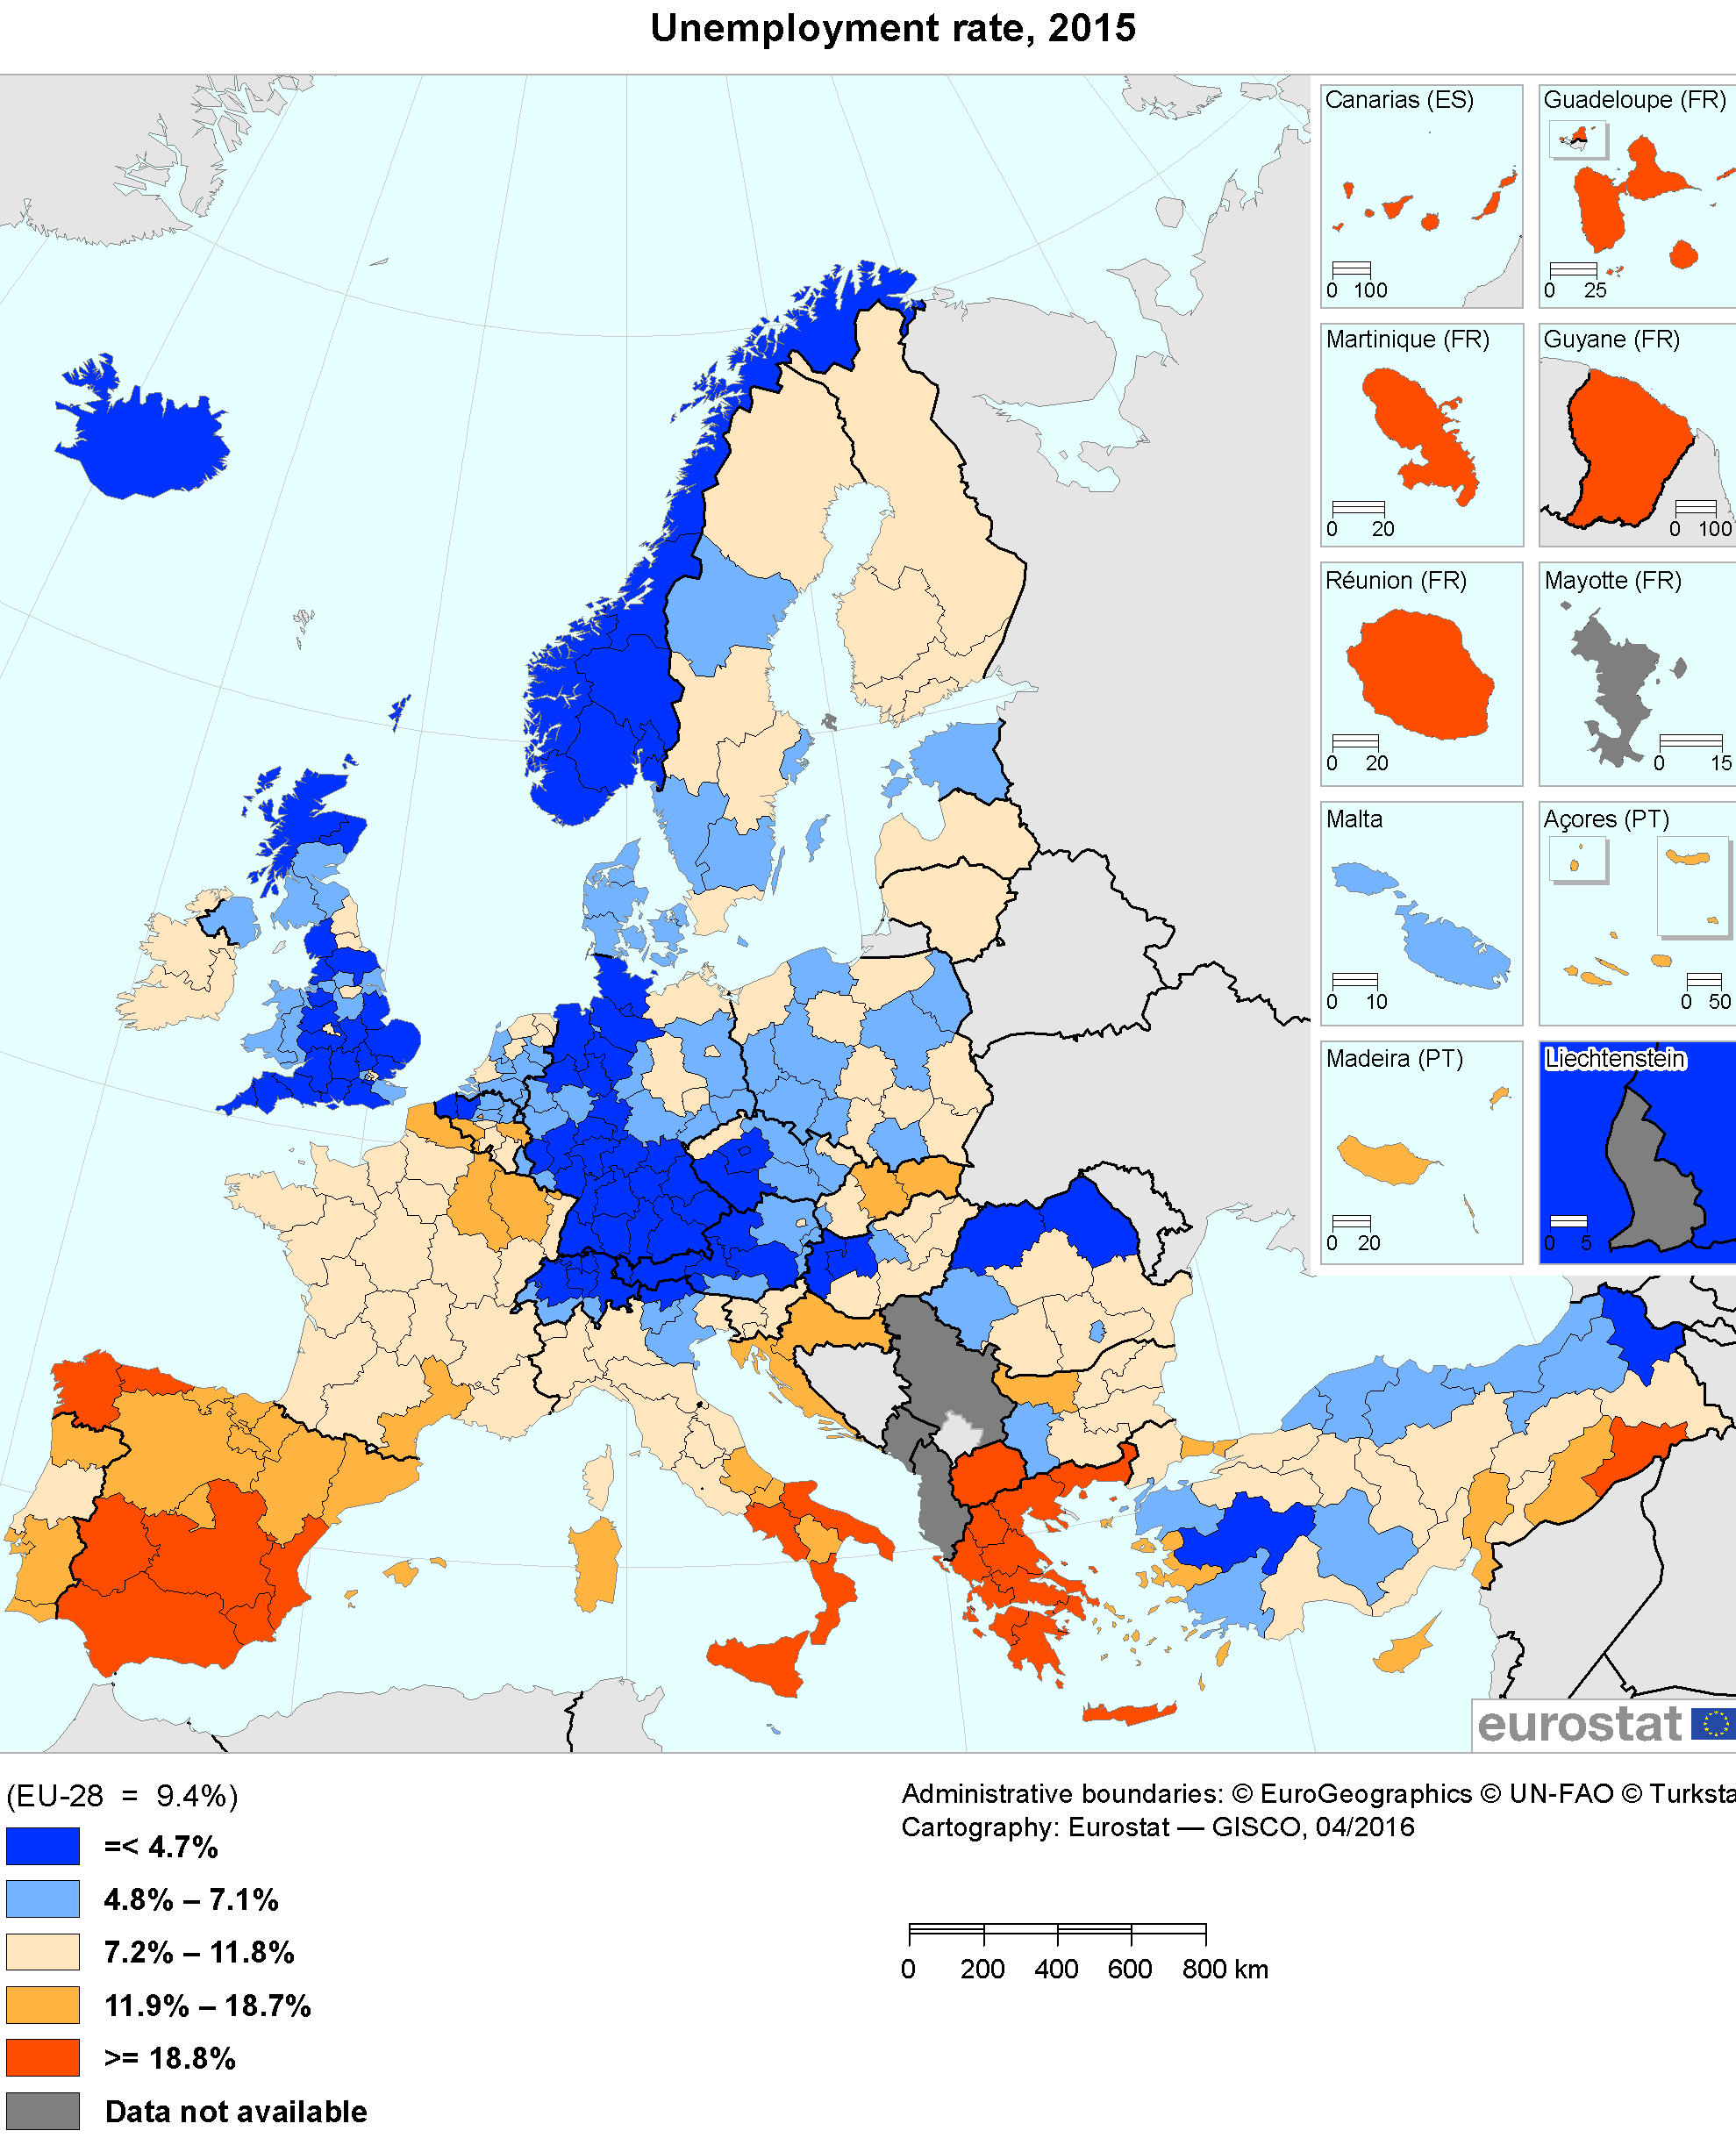
\includegraphics[height=6cm]{unemp}\\
\tiny{Source: Eurostat [\url{http://ec.europa.eu}]}

\column{.45\textwidth}
\centering
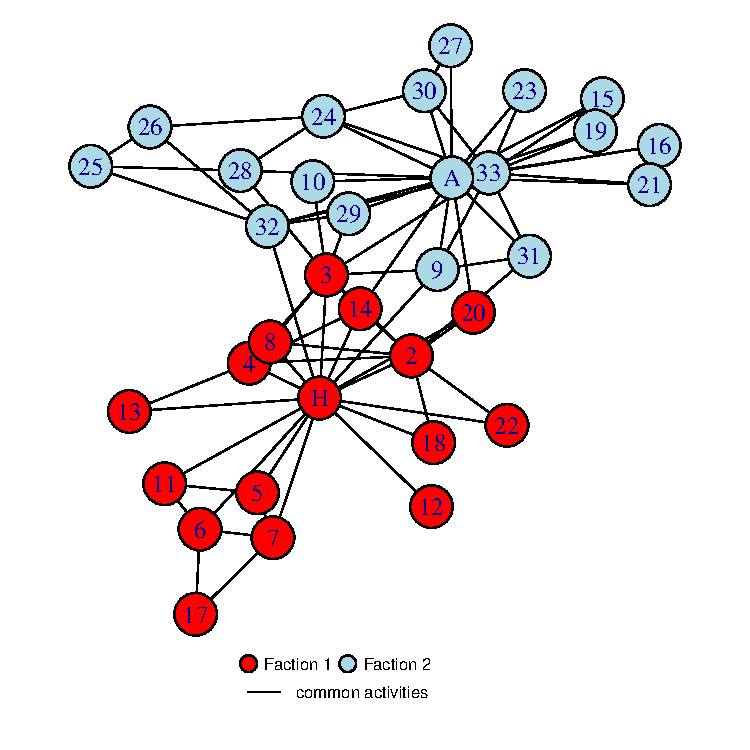
\includegraphics[height=6cm]{karate_l}\\
\tiny{Source: Karate club network (igraphdata) \cite{Zachary1977}}

\end{columns}

\end{frame}

%------------------------------------------------

\begin{frame}
\frametitle{\insertsection}
\framesubtitle{Maximise the data-ink ratio}

\begin{columns}[c]
\column{.45\textwidth} 
    \begin{itemize}
    \item Most of the `ink' used to print a graphic should represent {\color{blue}{data-information}}
    \item {\color{blue}{Data-ink}} is defined as the part of the graphic that we cannot erase without losing information
    \item {\color{blue}{Data-ink ratio}} is defined as the proportion of a graphic's ink devoted to the display of non-redundant information (data-ink)
\end{itemize}

\column{.45\textwidth}
\centering
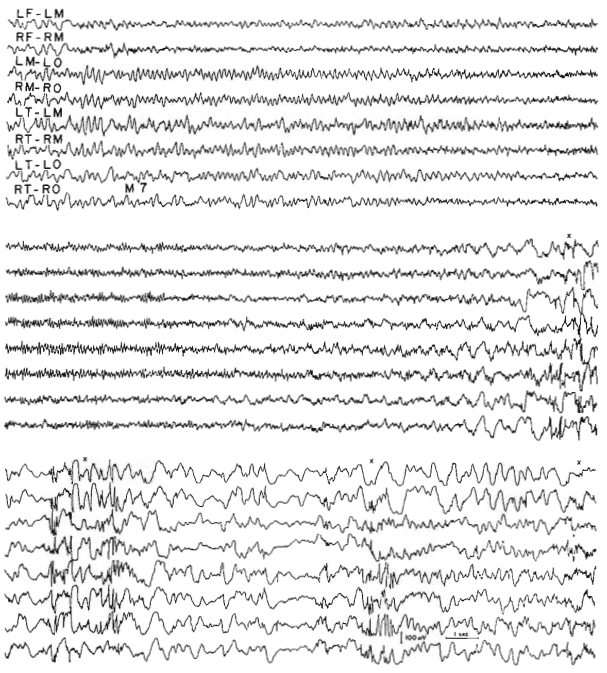
\includegraphics[width=5cm]{data_ink}\\
\tiny{Source: Fundamentals of electroencephalography \cite{Tufte2001}}
\end{columns}


\end{frame}

%------------------------------------------------

\begin{frame}
\frametitle{\insertsection}
\framesubtitle{Maximise the data-ink ratio}

\begin{columns}[t]
\column{.5\textwidth}
\\
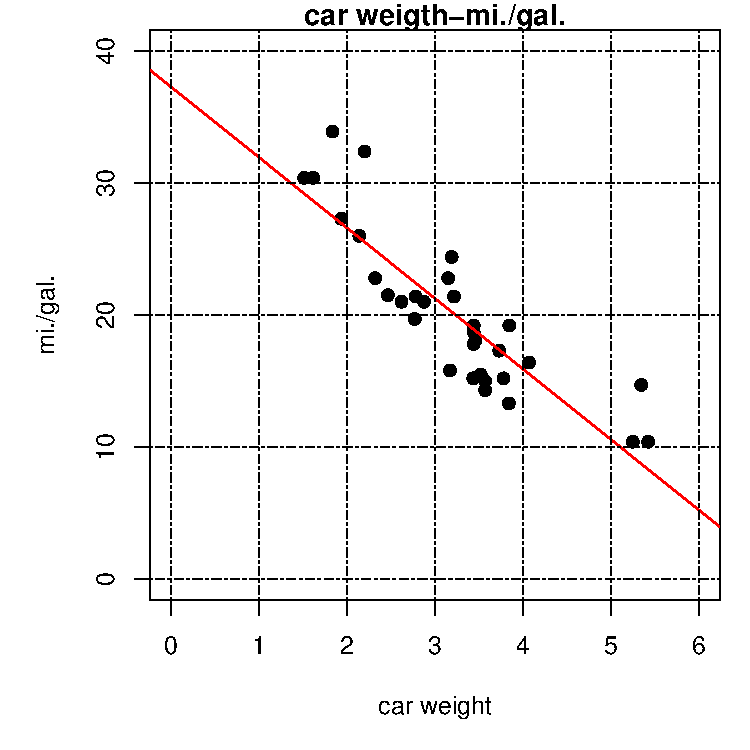
\includegraphics[width=0.9\linewidth]{data_ink_l}

\column{.5\textwidth}
\\
\onslide<2>{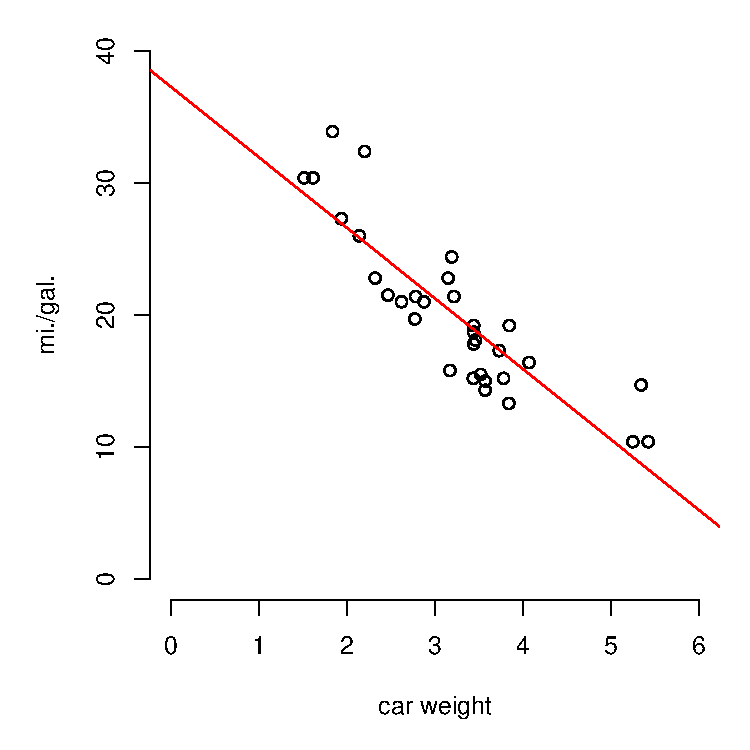
\includegraphics[width=0.9\linewidth]{data_ink_h}}

\end{columns}
  
\end{frame}

%------------------------------------------------

\begin{frame}
\frametitle{\insertsection}
\framesubtitle{Maximise the data-ink ratio}

\centering
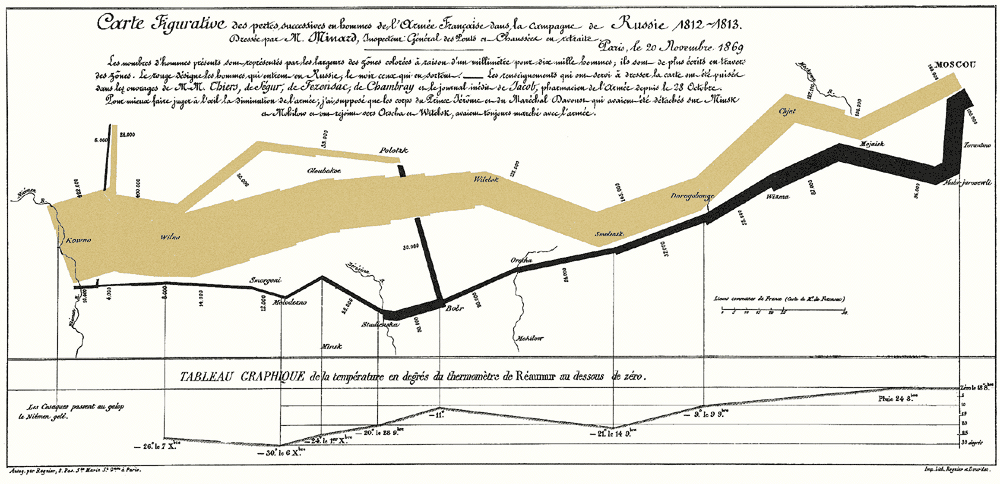
\includegraphics[width=0.9\linewidth]{minard}\\
\tiny{Source: Minard's visualisation of Napoleon's retreat from Moscow (\url{https://www.edwardtufte.com/tufte/minard})}
  
\end{frame}

%------------------------------------------------


\begin{frame}
\frametitle{\insertsection}
\framesubtitle{Maximise the data-ink ratio}

\begin{columns}
\column{.5\textwidth} 
\begin{itemize}
\item Maximise {\color{blue}{data-ink ratio}}
\item {\color{blue}{Erasing principles}} \cite{Tufte2001}
    \begin{itemize}
    \item Non-data-ink
    \item Redundant data-information
    \item Revise and edit
    \end{itemize}
\end{itemize}

\column{.5\textwidth}
\centering
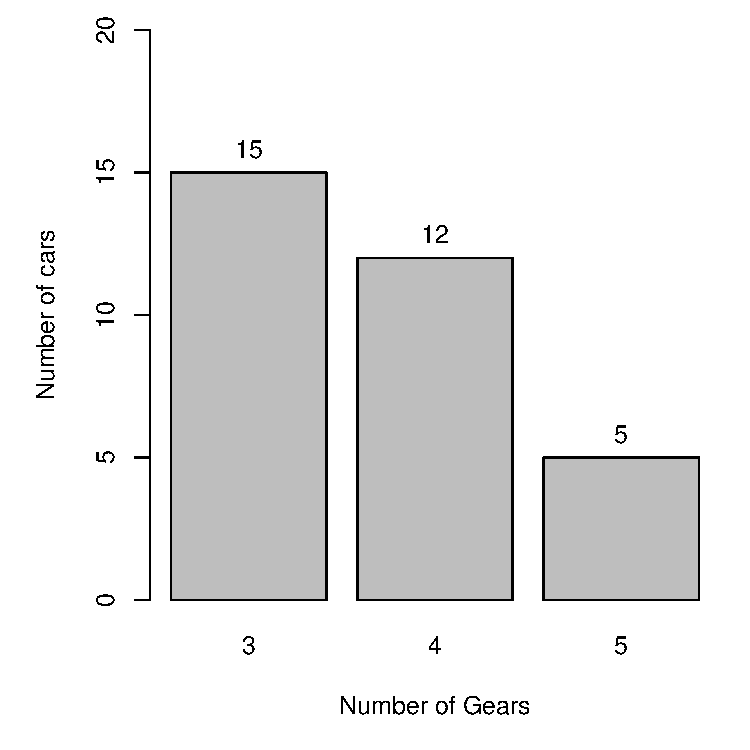
\includegraphics[width=5cm]{data_ink_b}\\

\end{columns}

  
\end{frame}


%NOTE =============
%== We can remove
%== Left line
%== Right line
%== The line of the height
%== The numbers
%== The bar color
%=================

%------------------------------------------------

\begin{frame}
\frametitle{\insertsection}
\framesubtitle{Graphical integrity}

\begin{columns}
\column{.5\textwidth} 
\begin{itemize}
    \item Graphics can {\color{blue}{distort}} underlying data
    \item Graphics can be used to {\color{blue}{deceive communication}}
    \item The visual representation may be consistent with data, while the {\color{blue}{perceived visual effect}} may deceive communication
\end{itemize}

\column{.5\textwidth}
\centering
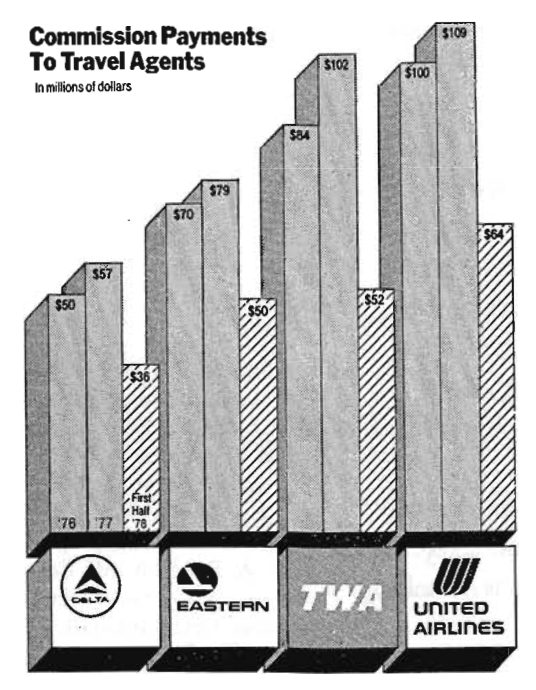
\includegraphics[width=5cm]{integrity_commission}\\
\tiny{Source: Commission payments to travel agents \cite{Tufte2001}}

\end{columns}

\end{frame}

%------------------------------------------------

\begin{frame}
\frametitle{\insertsection}
\framesubtitle{Graphical integrity}

\centering
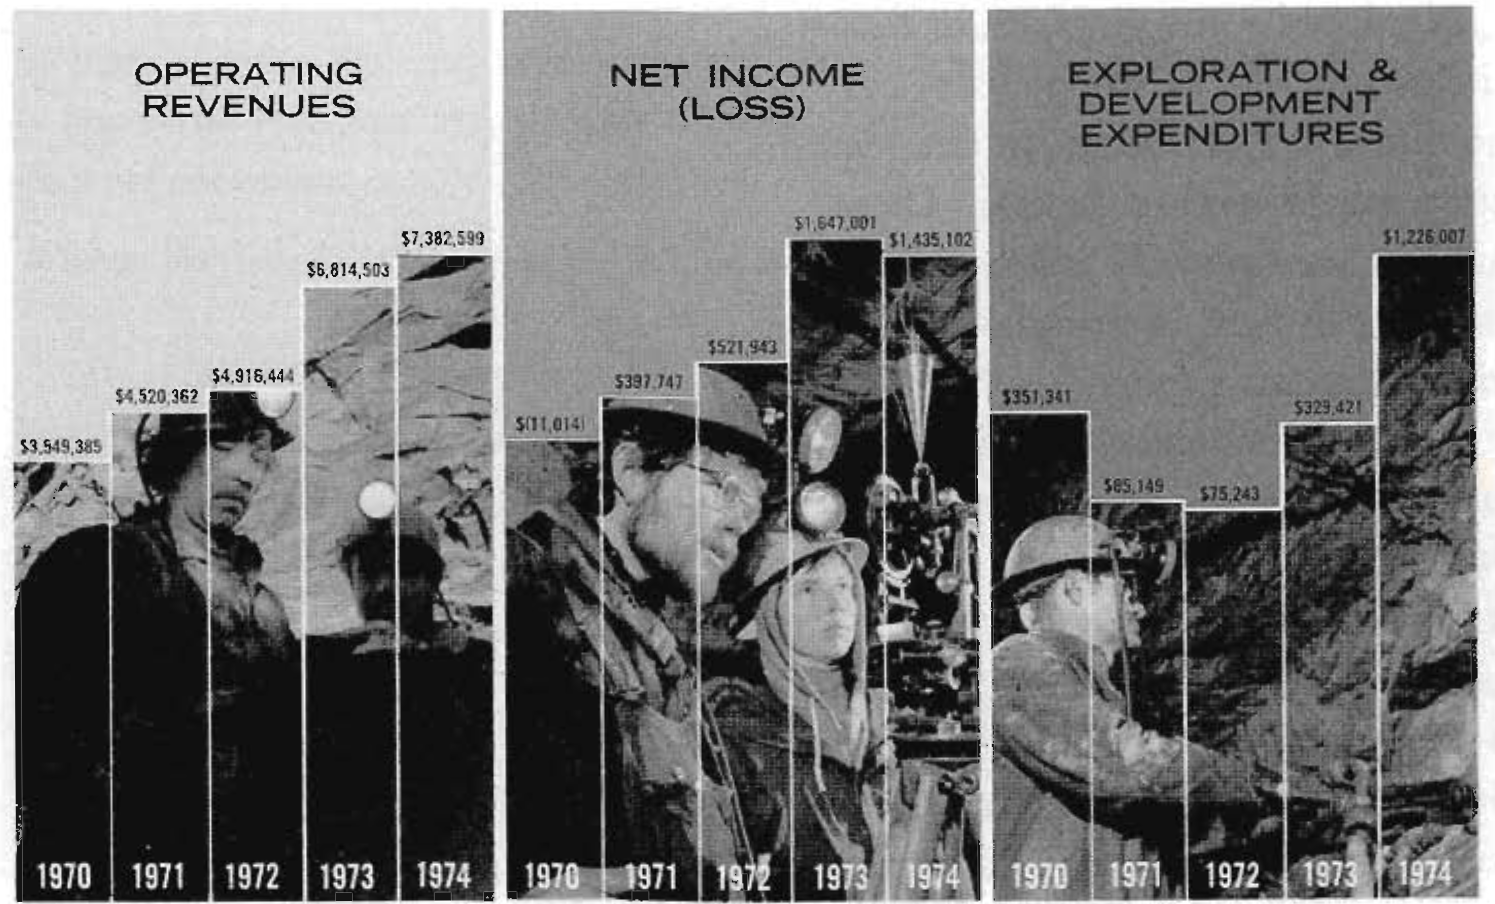
\includegraphics[width=10cm]{integrity_mines}\\
\tiny{Source: Annual report of a company \cite{Tufte2001}}

\end{frame}

%------------------------------------------------

\begin{frame}
\frametitle{\insertsection}
\framesubtitle{Graphical integrity}

\centering
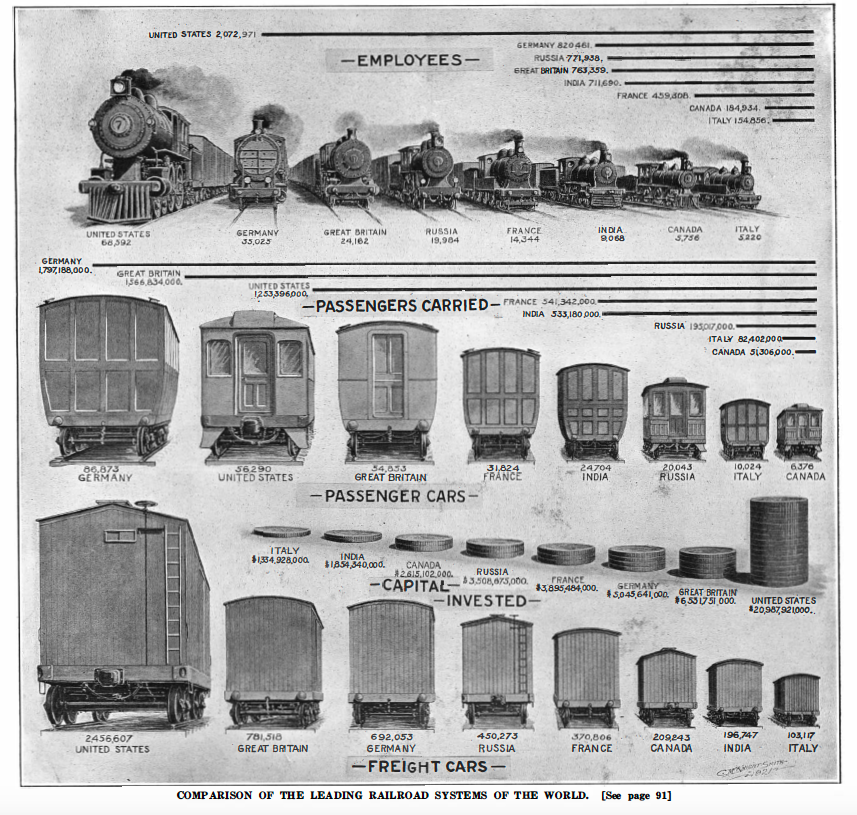
\includegraphics[height = 0.8\textheight]{SA_1921.png}\\
\tiny{Source: Scientific American (1921)}

\end{frame}

%------------------------------------------------

\begin{frame}
\frametitle{\insertsection}
\framesubtitle{Graphical integrity}

\centering
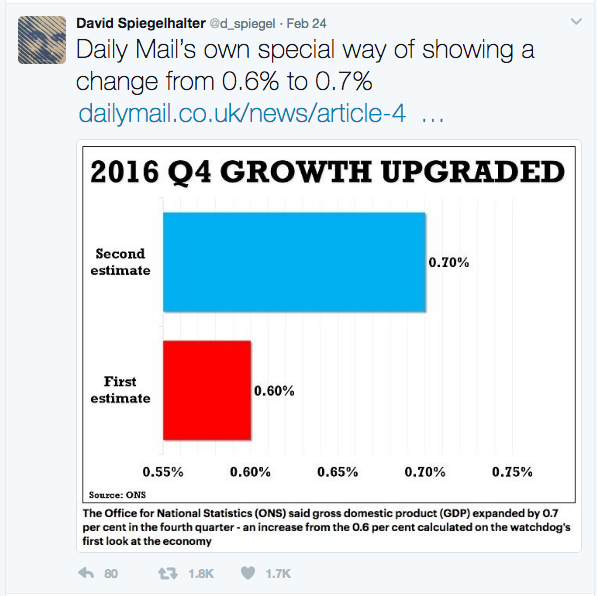
\includegraphics[width=7cm]{integrity}\\
\tiny{Source: Twitter (March, 2017)}

\end{frame}

%------------------------------------------------

\begin{frame}
\frametitle{\insertsection}
\framesubtitle{Graphical integrity}

\centering
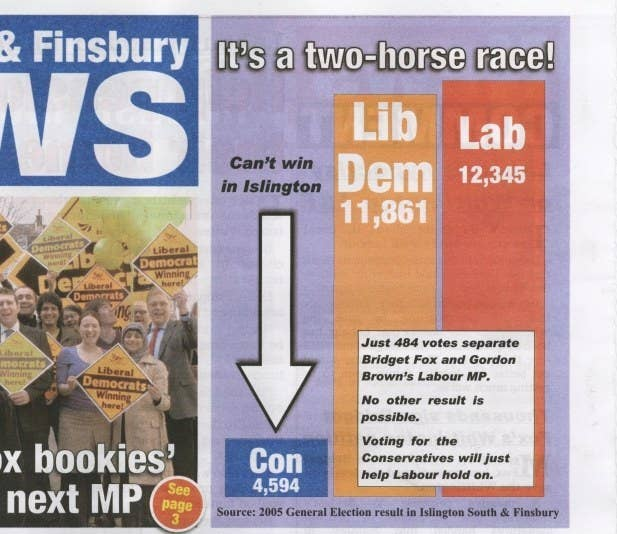
\includegraphics[width=7cm]{lib_dem.jpg}\\
\tiny{Source: Campaign ad in Islington South (https://electionleaflets.org/brb.html}

\end{frame}

%------------------------------------------------

\begin{frame}
\frametitle{\insertsection}
\framesubtitle{Graphical integrity}

\centering
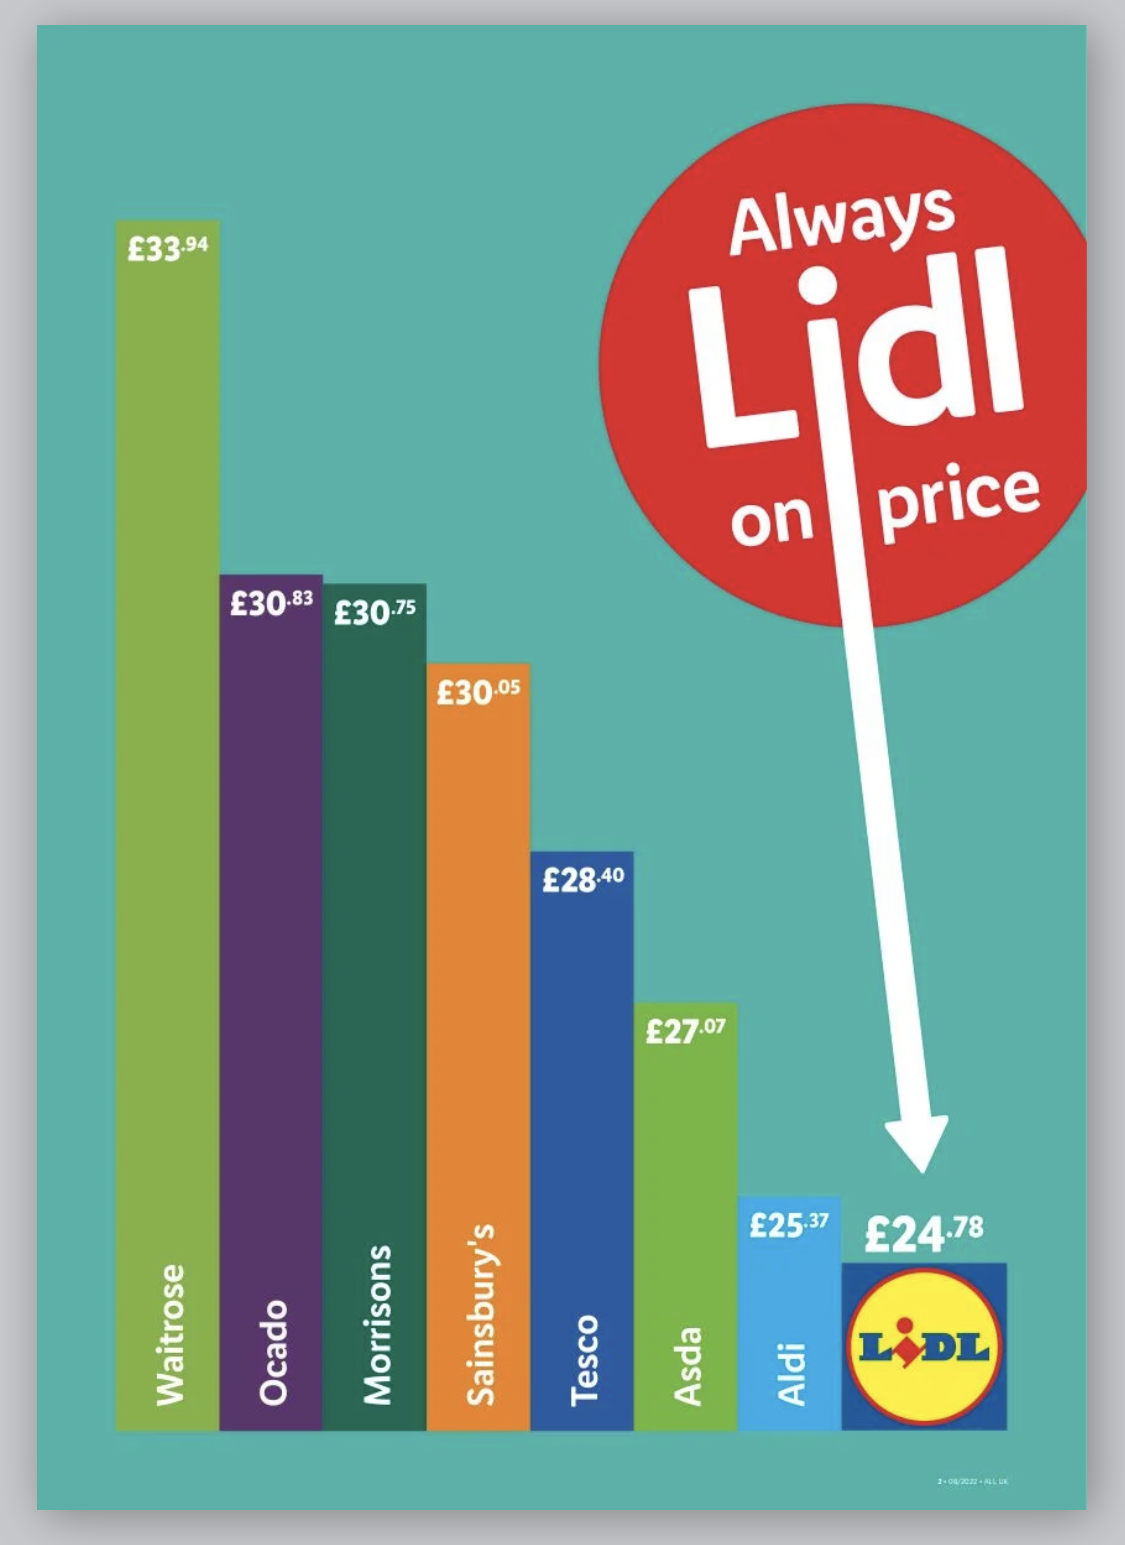
\includegraphics[width=5cm]{lidl_feb2022}\\
\tiny{Source: UK Lidl's leaflet (February 2022)}

\end{frame}

%------------------------------------------------


\begin{frame}
\frametitle{\insertsection}
\framesubtitle{Tools}

Some of the {\color{blue}{tools}} that can support the creation of infographics
\begin{itemize}
\item Microsoft Office (e.g.\ PowerPoint)
\item Google Documents (e.g. draw.io)
\item Adobe Creative Cloud 
\item Tableau (\url{www.tableau.com})
\item R (ggplot2)
\item Python, Java, D3js, etc.
\item ArcGIS, GoogleMaps, etc.
\item ...
\end{itemize}

\end{frame}

%------------------------------------------------




  
%=======================================================
%	The `good/bad infographic competition'
%=======================================================
\section{The good/bad infographic competition}
%------------------------------------------------
\bgroup
\setbeamercolor{background canvas}{bg = navyblue}
\begin{frame}[plain]{}
\begin{center}
\color{white}{\Huge\insertsection}
\end{center}
\end{frame}
\egroup

%------------------------------------------------

\begin{frame}
\frametitle{\insertsection}

\begin{enumerate}
\item Groups of 4 students (randomly selected)
\item Identify a {\color{dkgreen}{good example}} and a {\color{red}{bad example}}  of infographics 
\item Every group has a leader (name in bold) in charge of the submission
\item Please do send your examples on Canvas by {\color{orange}{21 March 2022}}
\item Groups will showcase their examples during the lecture in Week
\item We will then vote for the best {\color{dkgreen}{`good infographic'}} and for the best {\color{red}{`bad infographic'}}
\end{enumerate}


\end{frame}

%------------------------------------------------

\begin{frame}
\frametitle{\insertsection}


\begin{table}
\begin{tabular}{ll}
\toprule
Group 1: \textbf{Ross}, Johanna, Samuel, Maria Belen\\
\\
Group 2: \textbf{Maria Fernanda}, Poojani, Saradha, Charunan\\
\\
Group 3: \textbf{Evi}, Ananya, Noemie, Harry\\
\\				
Group 4: \textbf{Perizat}, America, Ayesha, Oscar\\
\\
Group 5: \textbf{Jongho}, Daniela, Tanya, Anas\\
\bottomrule
\end{tabular}
\end{table}

\end{frame}




%=======================================================
%	Network visualisation
%=======================================================
\section{Network visualisation}
%------------------------------------------------

\bgroup
\setbeamercolor{background canvas}{bg = navyblue}
\begin{frame}[plain]{}
\begin{center}
\color{white}{\Huge\insertsection}
\end{center}
\end{frame}
\egroup

%------------------------------------------------
\begin{frame}
\frametitle{\insertsection}

We can convey additional information through
\begin{itemize}
\item {\color{blue}{Nodes}}: size, colour, and shape
\item {\color{blue}{Edges}}: width, colour, and line type
\item {\color{blue}{Layout}}: position of nodes
\end{itemize}
 
\end{frame}

%------------------------------------------------

\begin{frame}
\frametitle{\insertsection}
\framesubtitle{Layout}

Let's generate a network $G(N, E)$ where:
\begin{itemize}
\item $N=100$
\item $x_{ij} = 1$ with $p=0.02$
\end{itemize}
 
\end{frame}

%------------------------------------------------

\begin{frame}
\frametitle{\insertsection}
\framesubtitle{Layout: Random}

\centering
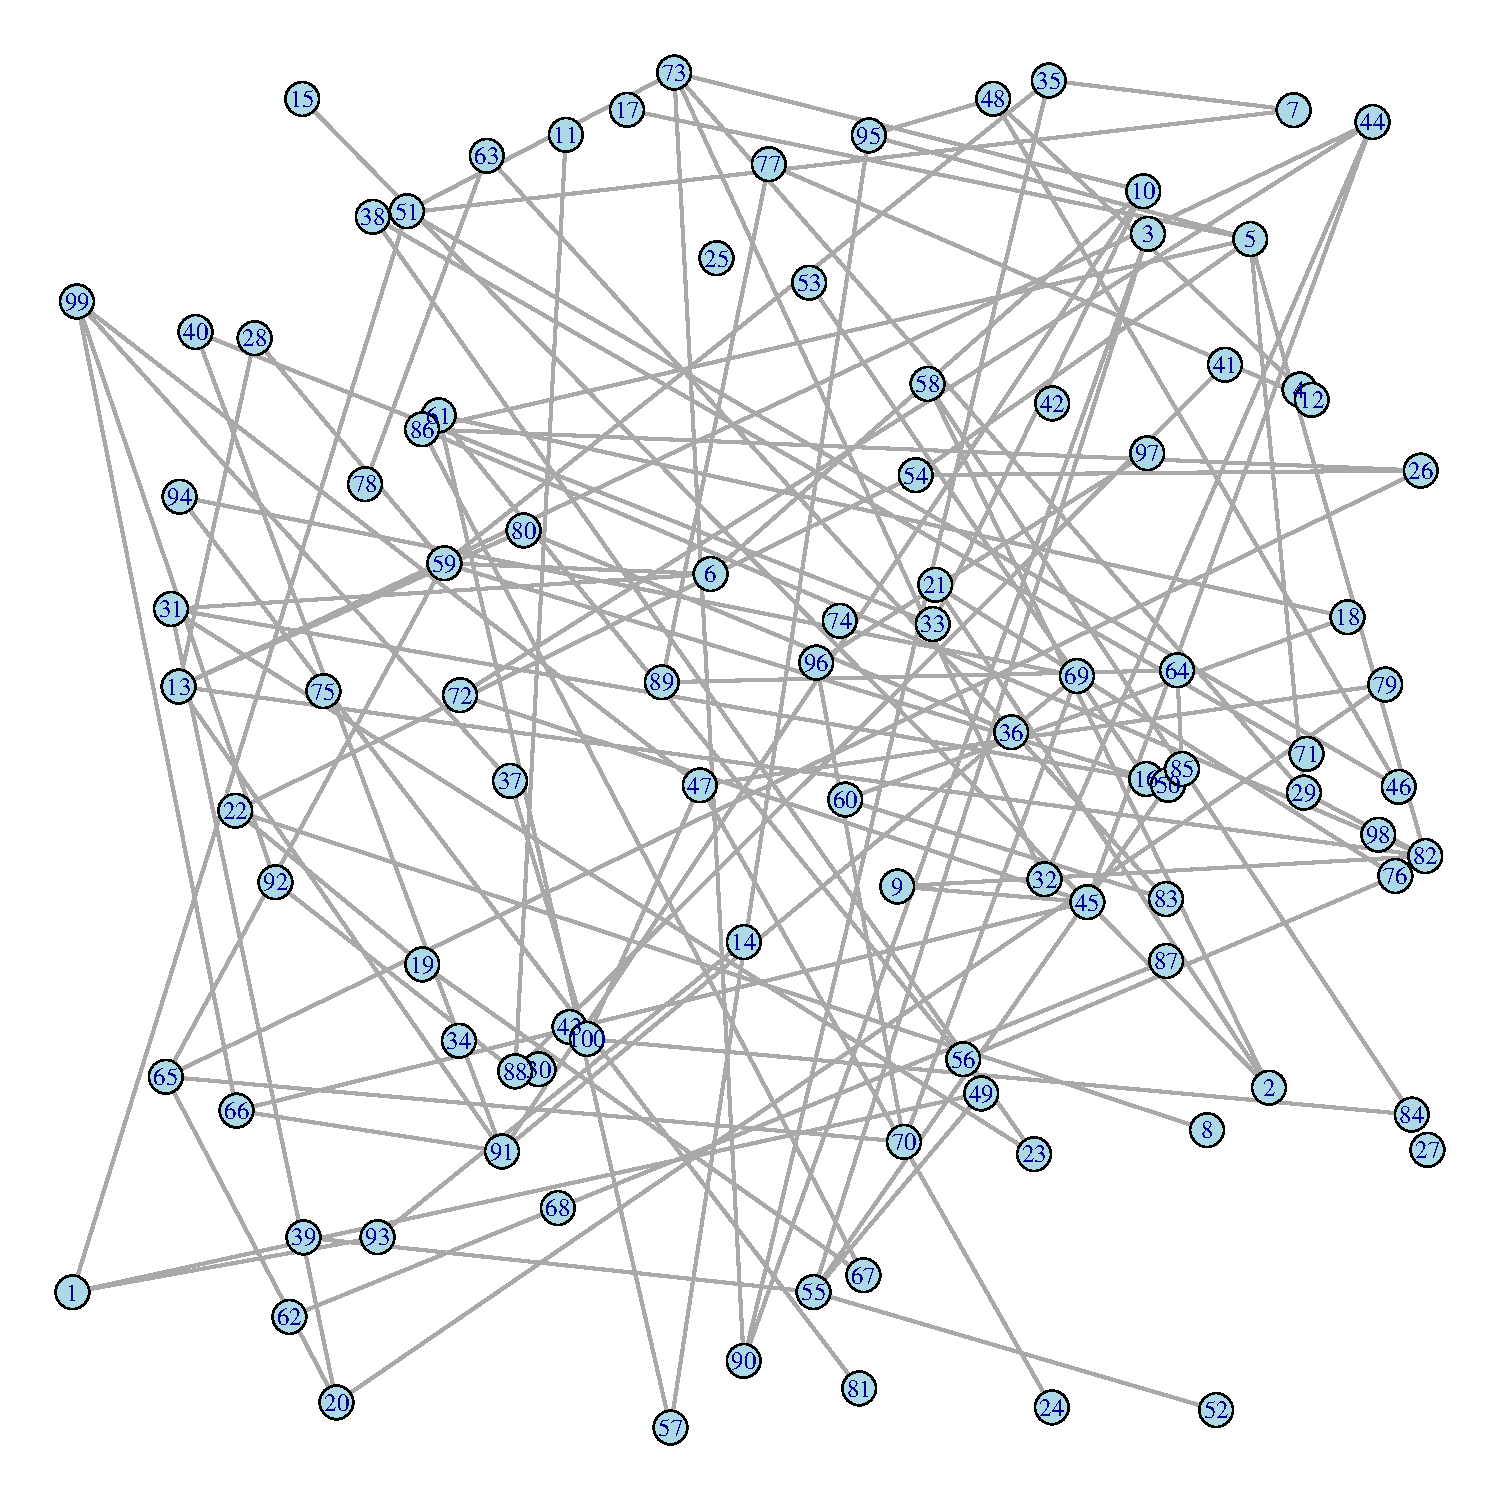
\includegraphics[height=0.85\textheight]{random}

\end{frame}

%------------------------------------------------

\begin{frame}
\frametitle{\insertsection}
\framesubtitle{Layout}

\begin{columns}
\column{.45\textwidth} 
\begin{itemize}
\item A network visualization should provide a relatively clear view of the {\color{blue}{structure of the network}} (e.g.\ central nodes)
\item This requires positioning nodes in a 2D (or 3D) space according to {\color{blue}{certain criteria/rules}}
\end{itemize}

\column{.5\textwidth} 
\centering
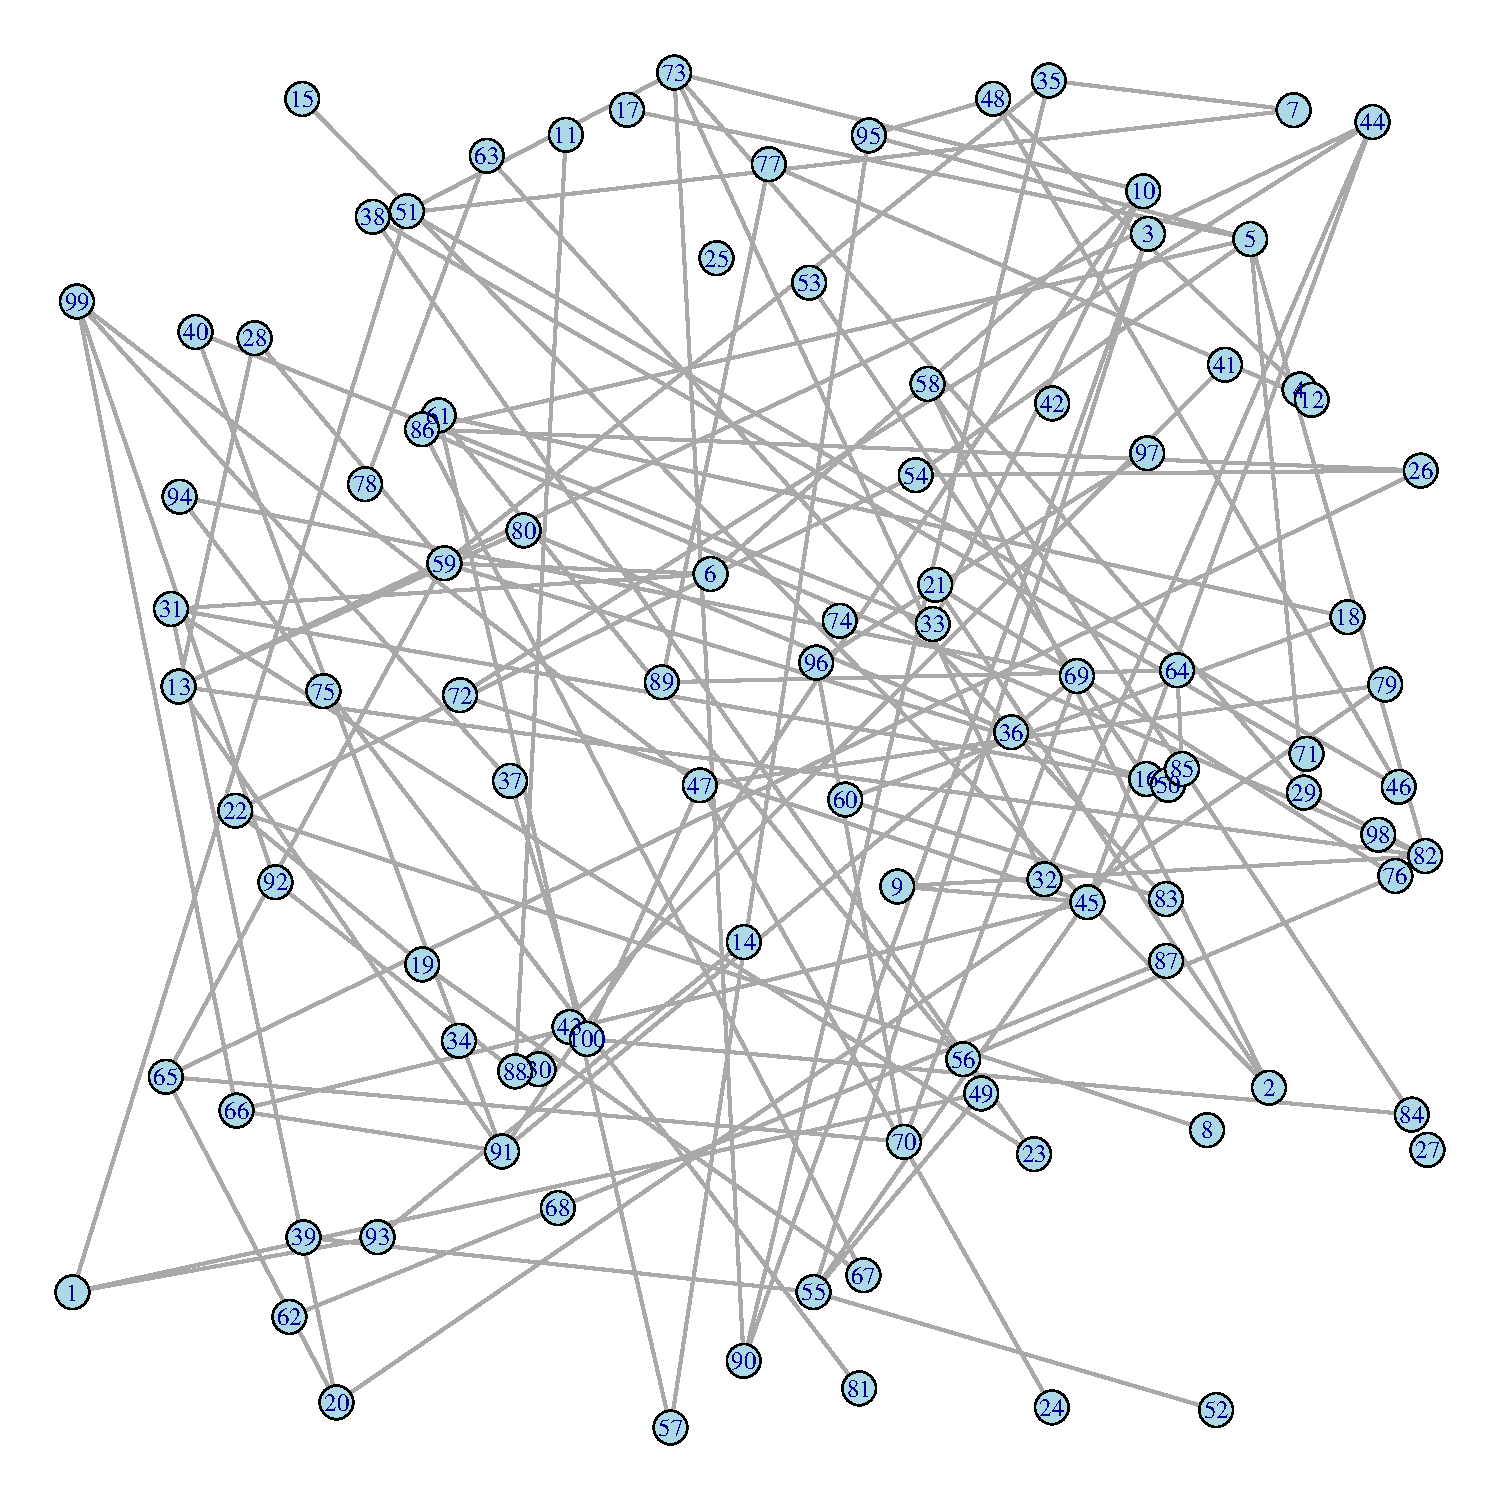
\includegraphics[width=5cm]{random}\\
   
\end{columns}

\end{frame}

%------------------------------------------------

\begin{frame}
\frametitle{\insertsection}
\framesubtitle{Layout: Circle}

\centering
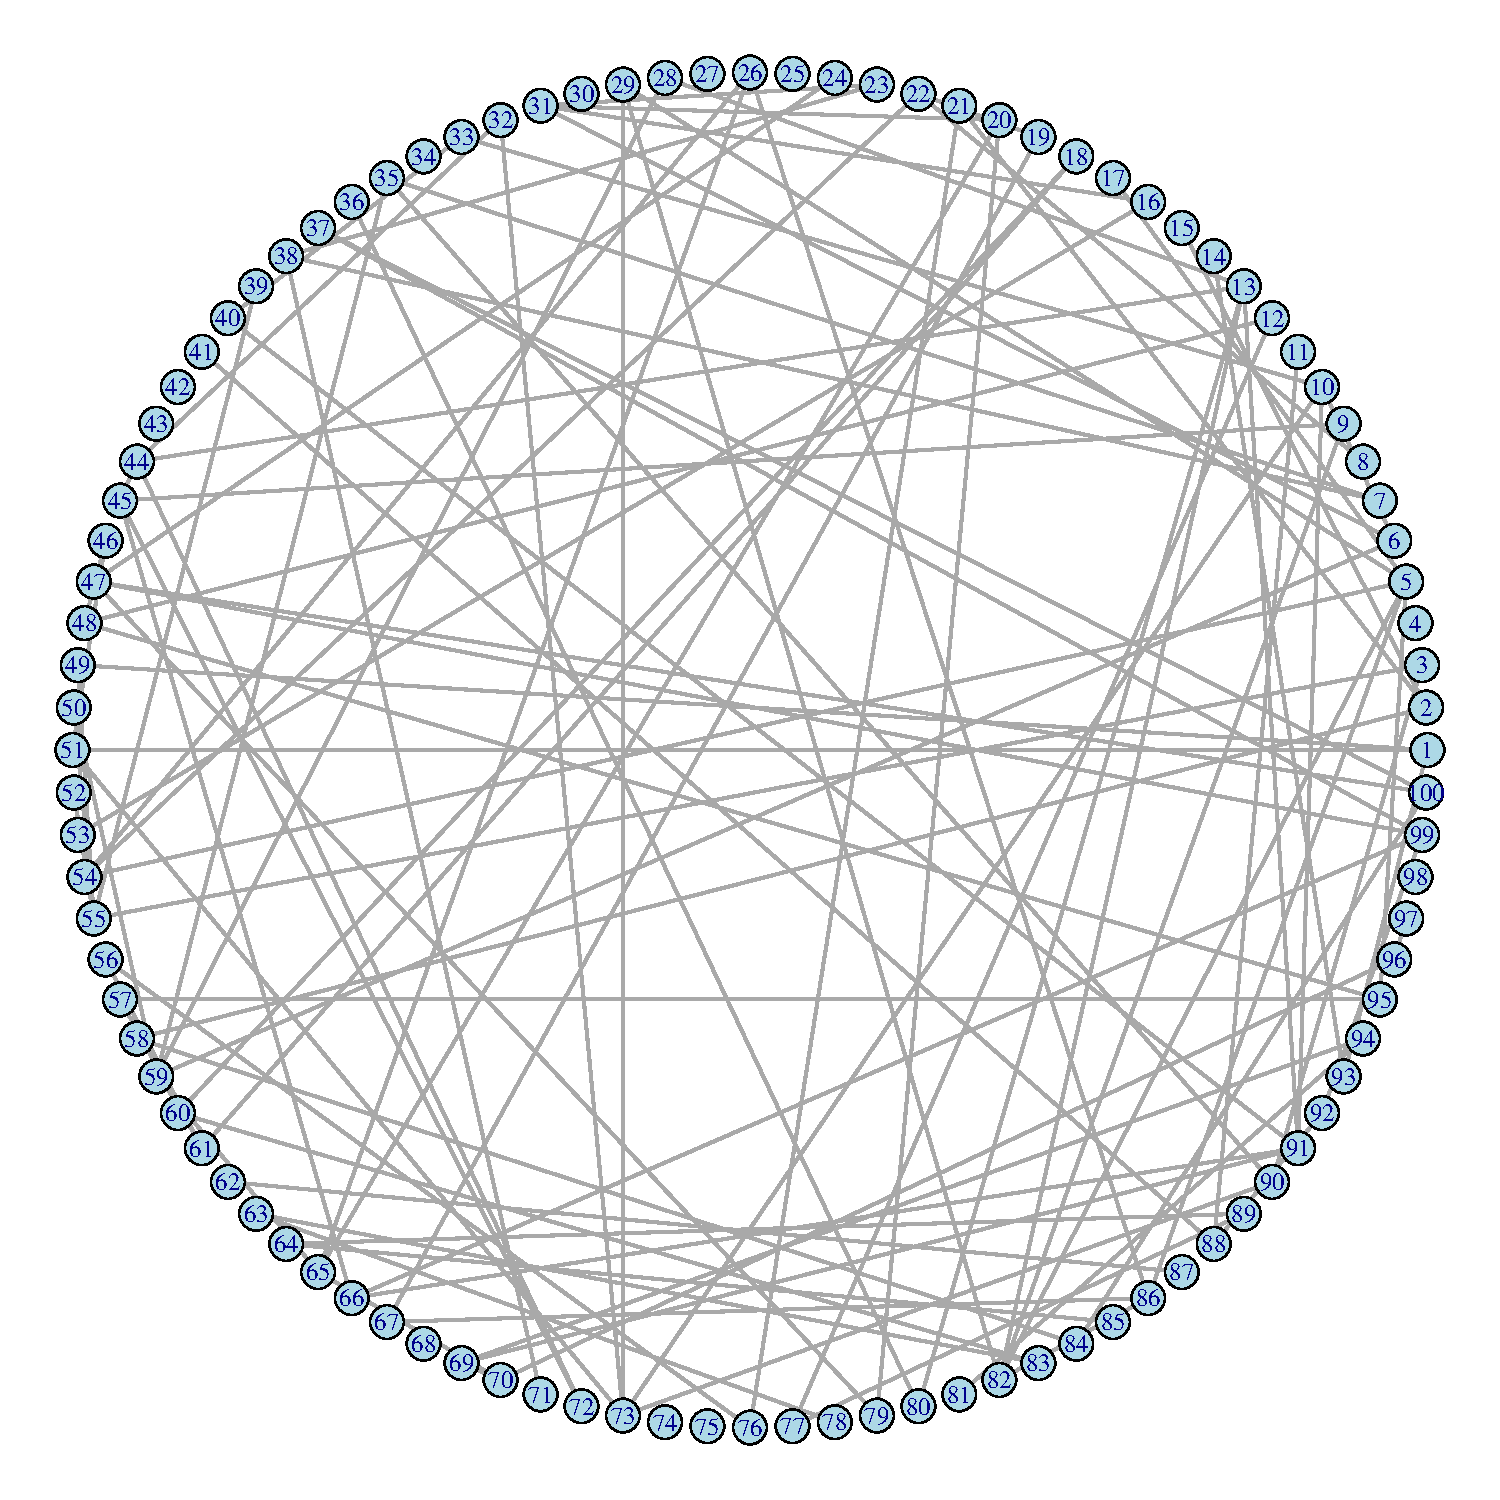
\includegraphics[height=0.85\textheight]{circle}

\end{frame}

%------------------------------------------------

\begin{frame}
\frametitle{\insertsection}
\framesubtitle{Layout: Grid}

\centering
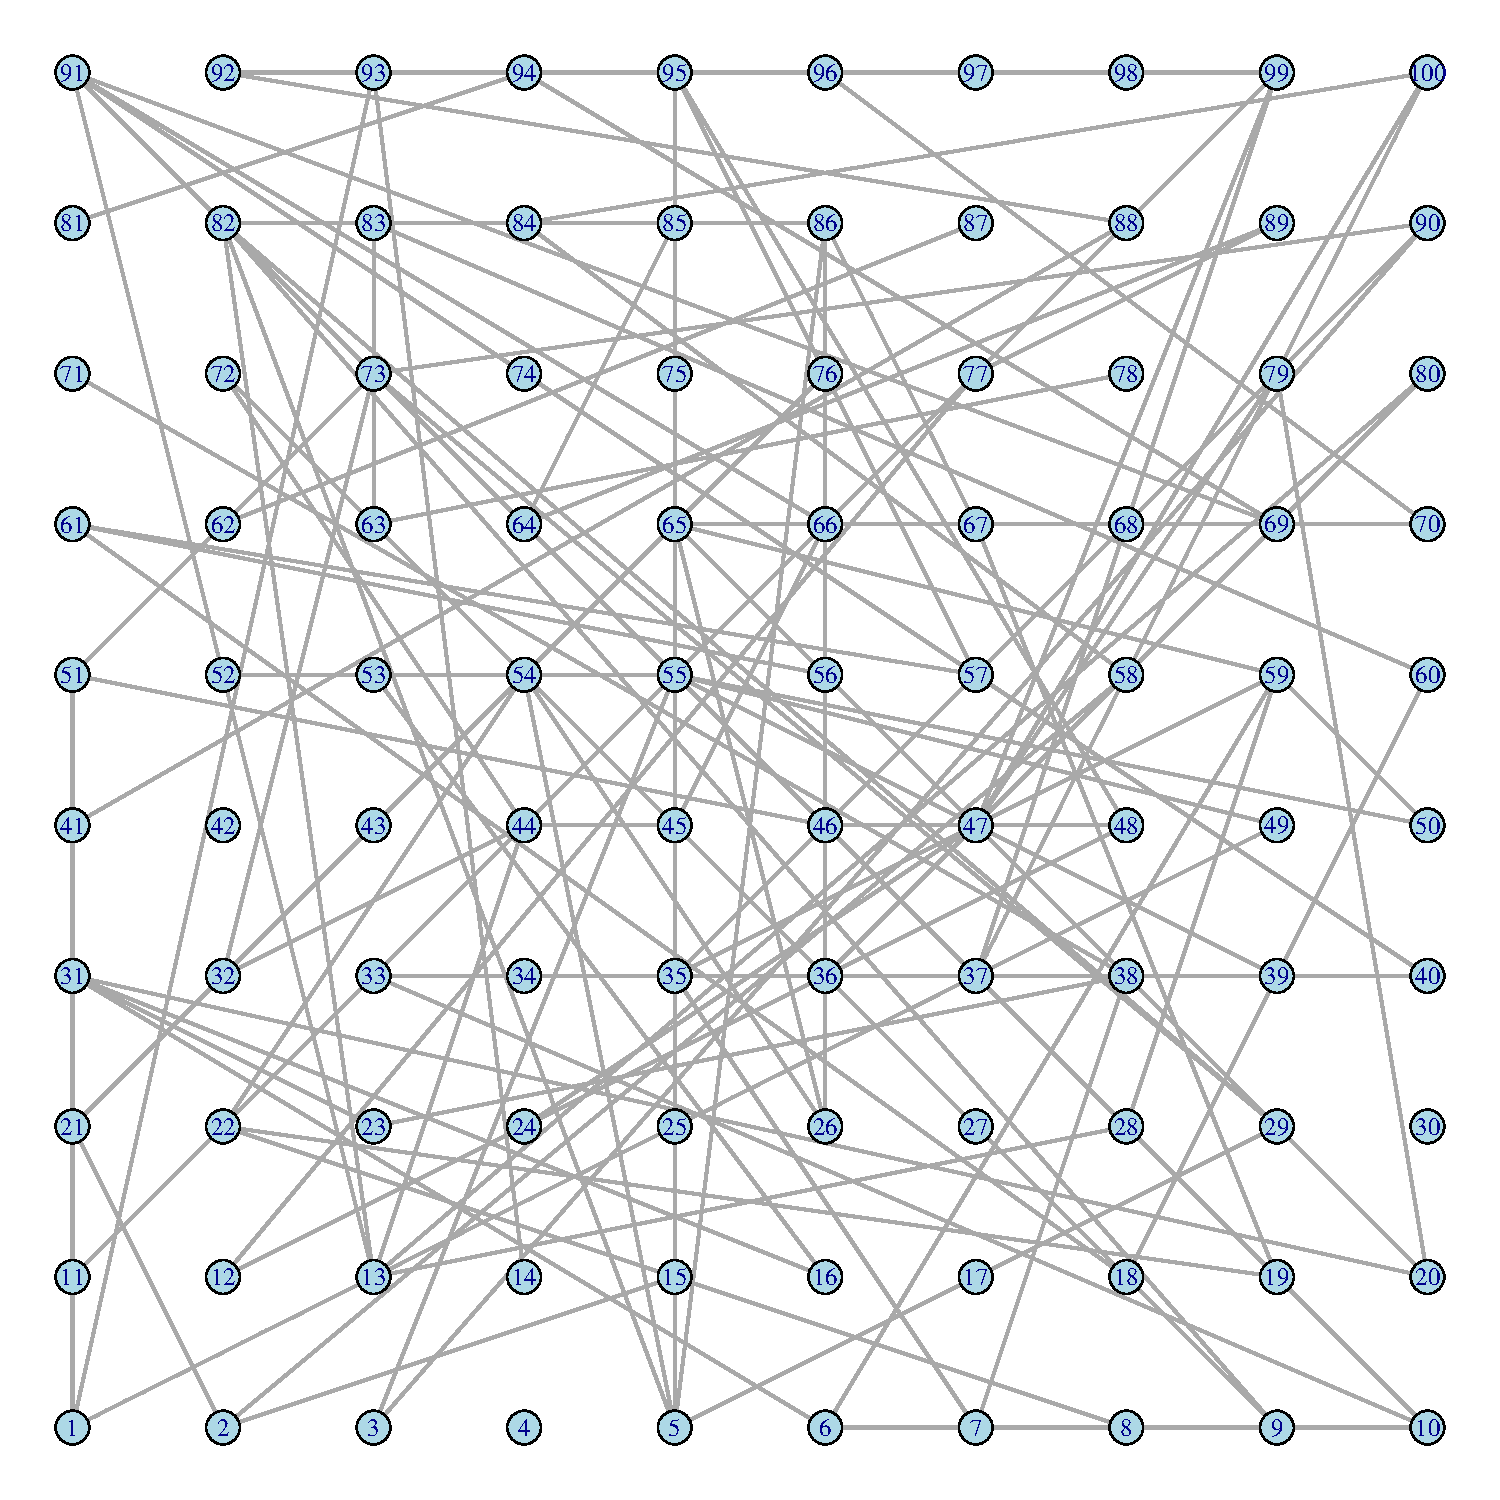
\includegraphics[height=0.85\textheight]{grid}
 
\end{frame}
%------------------------------------------------

\begin{frame}
\frametitle{\insertsection}
\framesubtitle{Layout in igraph}


\begin{columns}
\column{.5\textwidth}
\centering
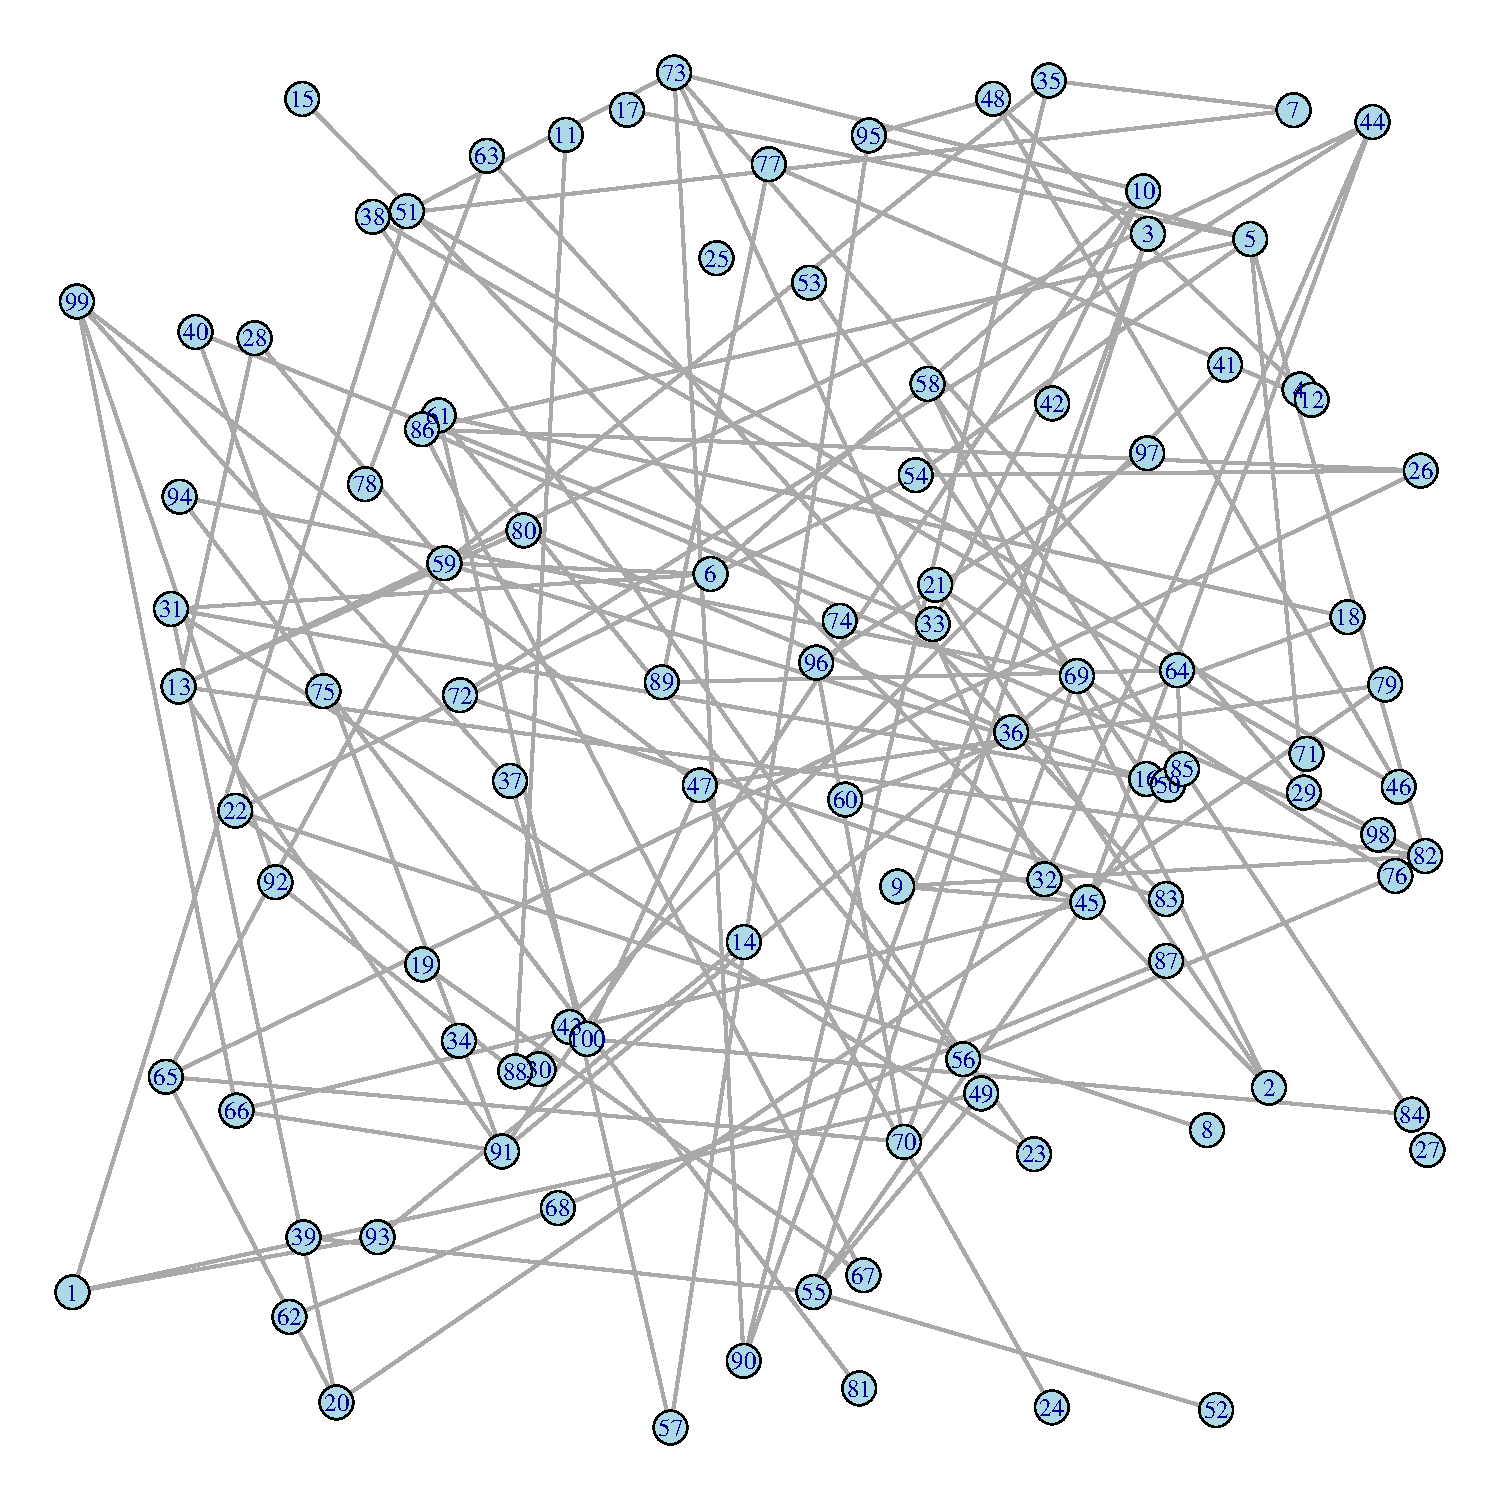
\includegraphics[width=0.4\linewidth]{random}\\
\lstinputlisting[language=R, firstline=15, lastline=23]{handouts_script/L7_script_handouts.R}

\column{.5\textwidth}
\centering
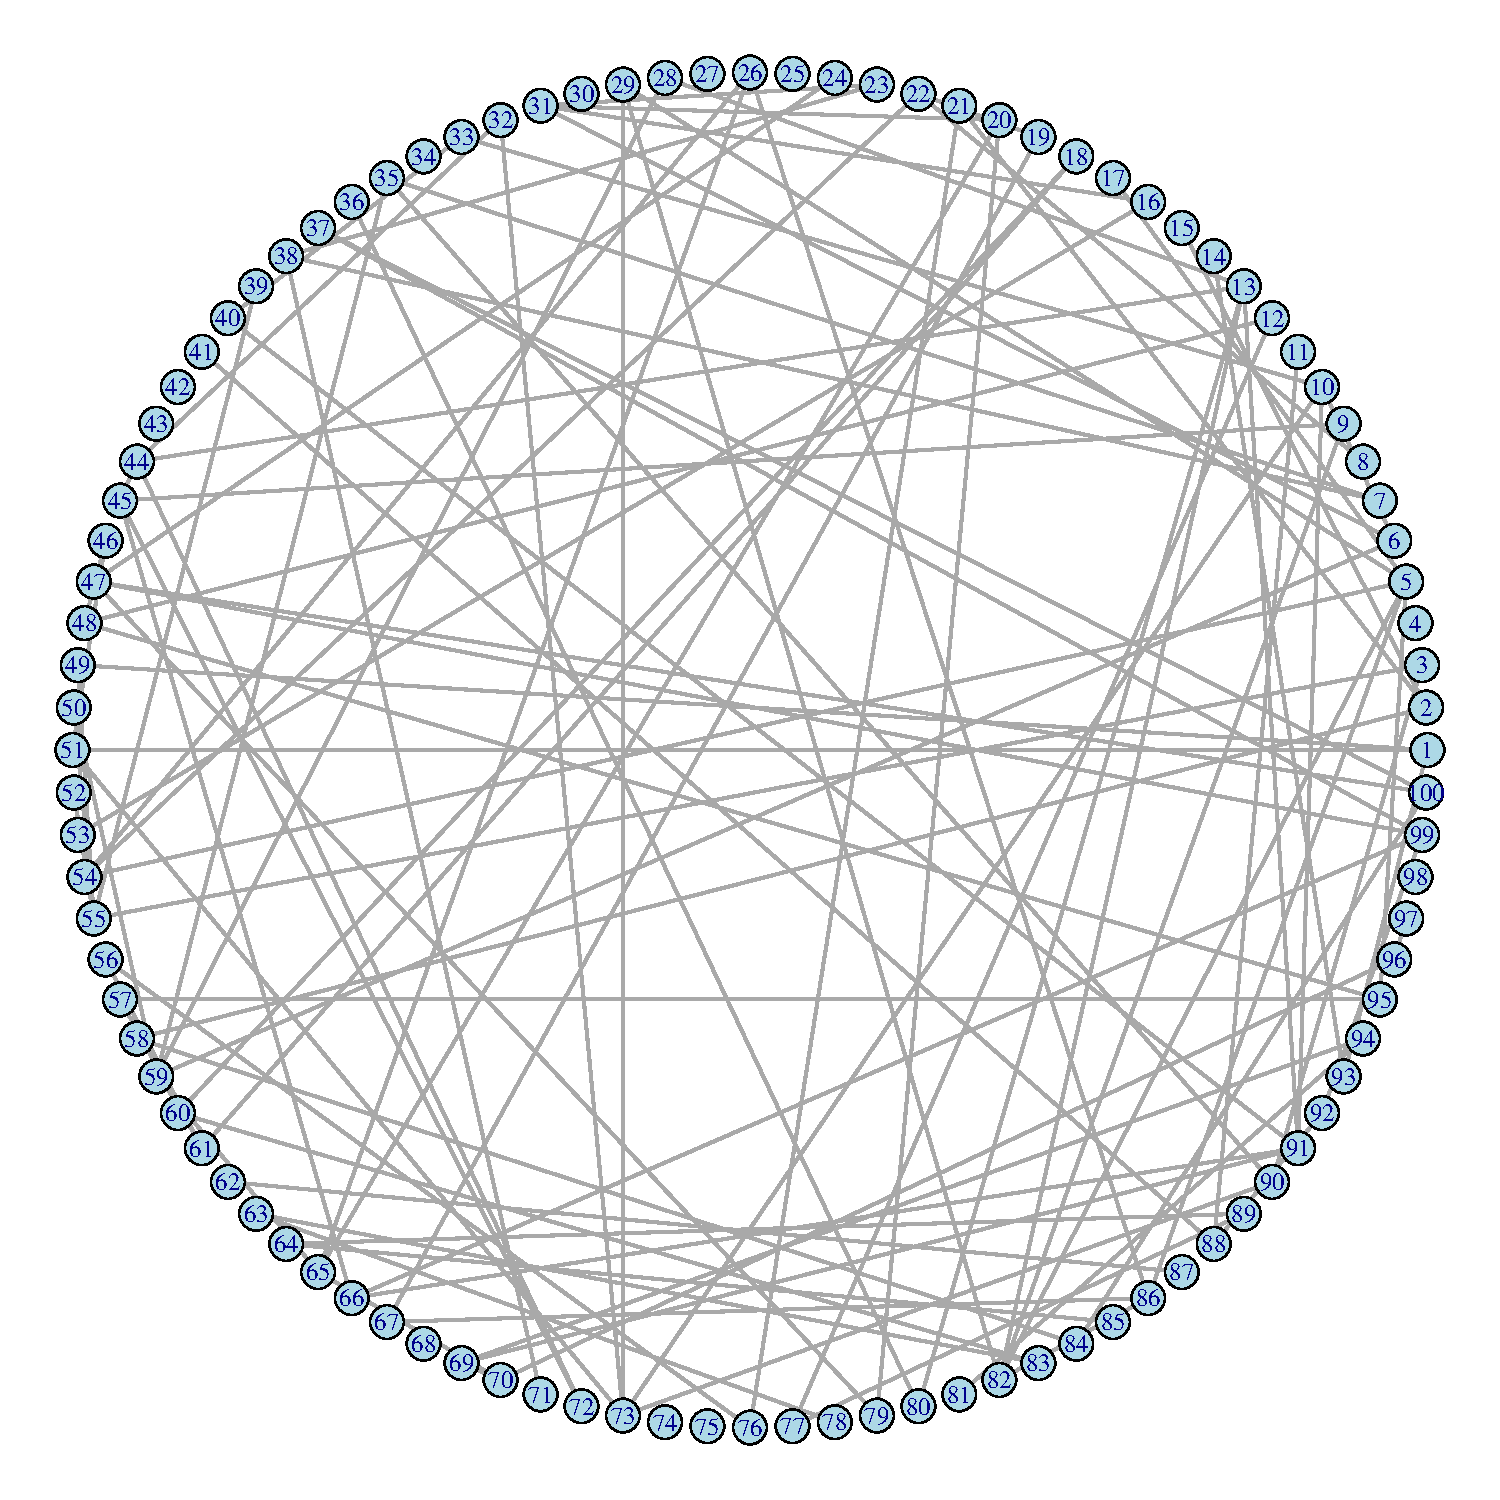
\includegraphics[width=0.4\linewidth]{circle}\\
\lstinputlisting[language=R, firstline=27, lastline=31]{handouts_script/L7_script_handouts.R}


\centering
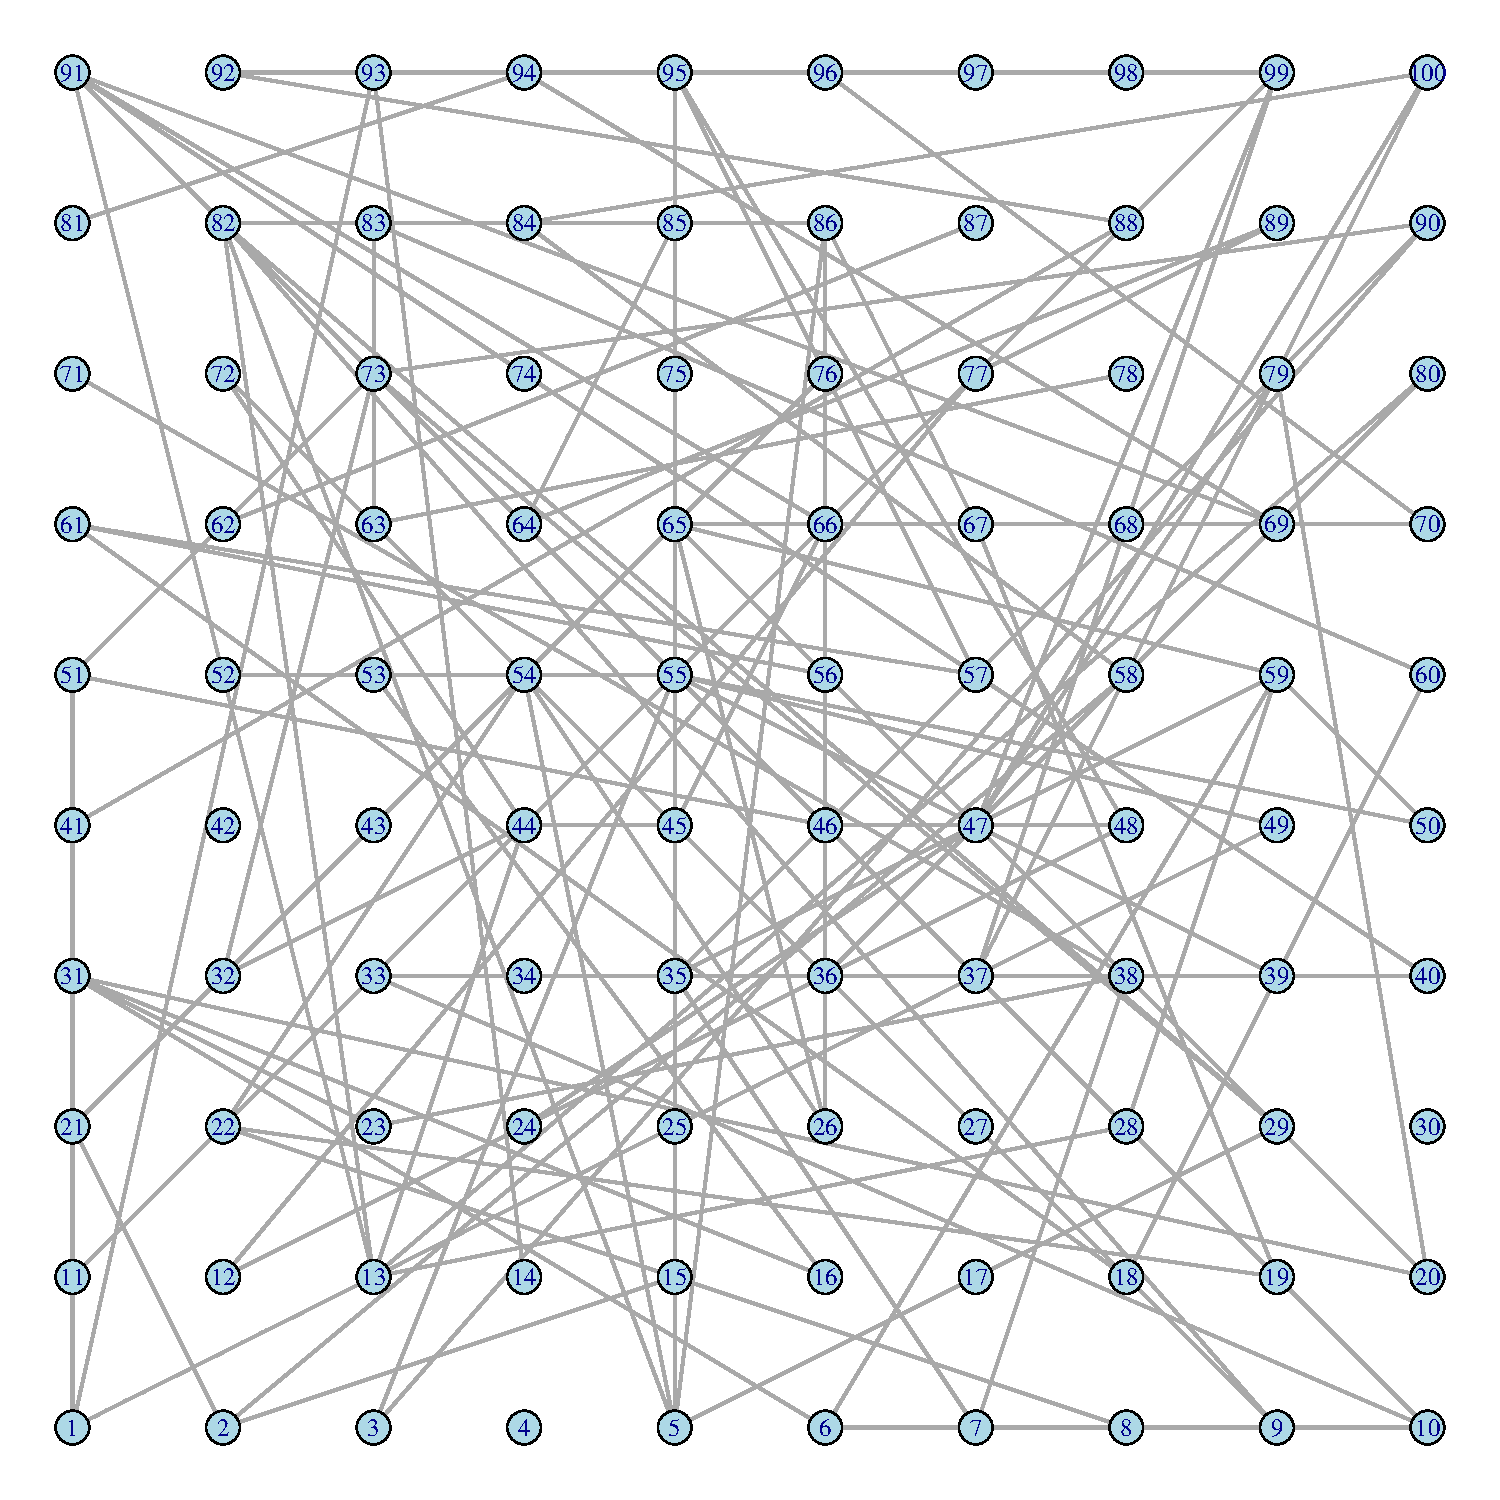
\includegraphics[width=0.4\linewidth]{grid}\\
\lstinputlisting[language=R, firstline=35, lastline=39]{handouts_script/L7_script_handouts.R}
\end{columns}

\end{frame}

%------------------------------------------------

\begin{frame}
\frametitle{\insertsection}
\framesubtitle{Layout algorithms}


\begin{itemize}
\item A variety of {\color{blue}{layout algorithms}} have been developed to improve the layout of nodes and therefore network visualisations
\item We focus on {\color{blue}{force-directed}} algorithms: The layout of a network is defined using the information contained within the {\color{blue}{structure of the network}} itself

    \begin{itemize}
    \item Kamada-Kawai
    \item Fruchterman and Reingold
    \end{itemize}
    
\end{itemize}

\vspace{0.5cm}




\end{frame}
%------------------------------------------------

\begin{frame}
\frametitle{\insertsection}
\framesubtitle{Layout: Kamada-Kawai}


{\color{blue}{\cite{Kamada1989}}}
    \begin{itemize}
    \item Ties as {\color{blue}{springs}} exerting attraction and repulsion forces between nodes
    \item {\color{blue}{Length of spring}}: proportional to the shortest distance between two nodes
    \item {\color{blue}{Strength of the spring}} (i.e.\ repulsion and attraction forces): inversely proportional to the square of the shortest distance between two nodes
    \end{itemize}

\medskip
\medskip

\centering
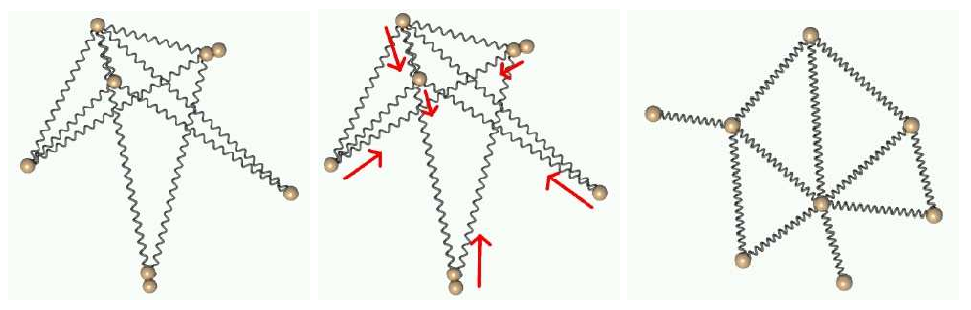
\includegraphics[width=8cm]{spring}\\
\tiny{Source: \cite{Kobourov2012}}

\end{frame}

%------------------------------------------------

\begin{frame}
\frametitle{\insertsection}
\framesubtitle{Layout: Kamada-Kawai}

\centering
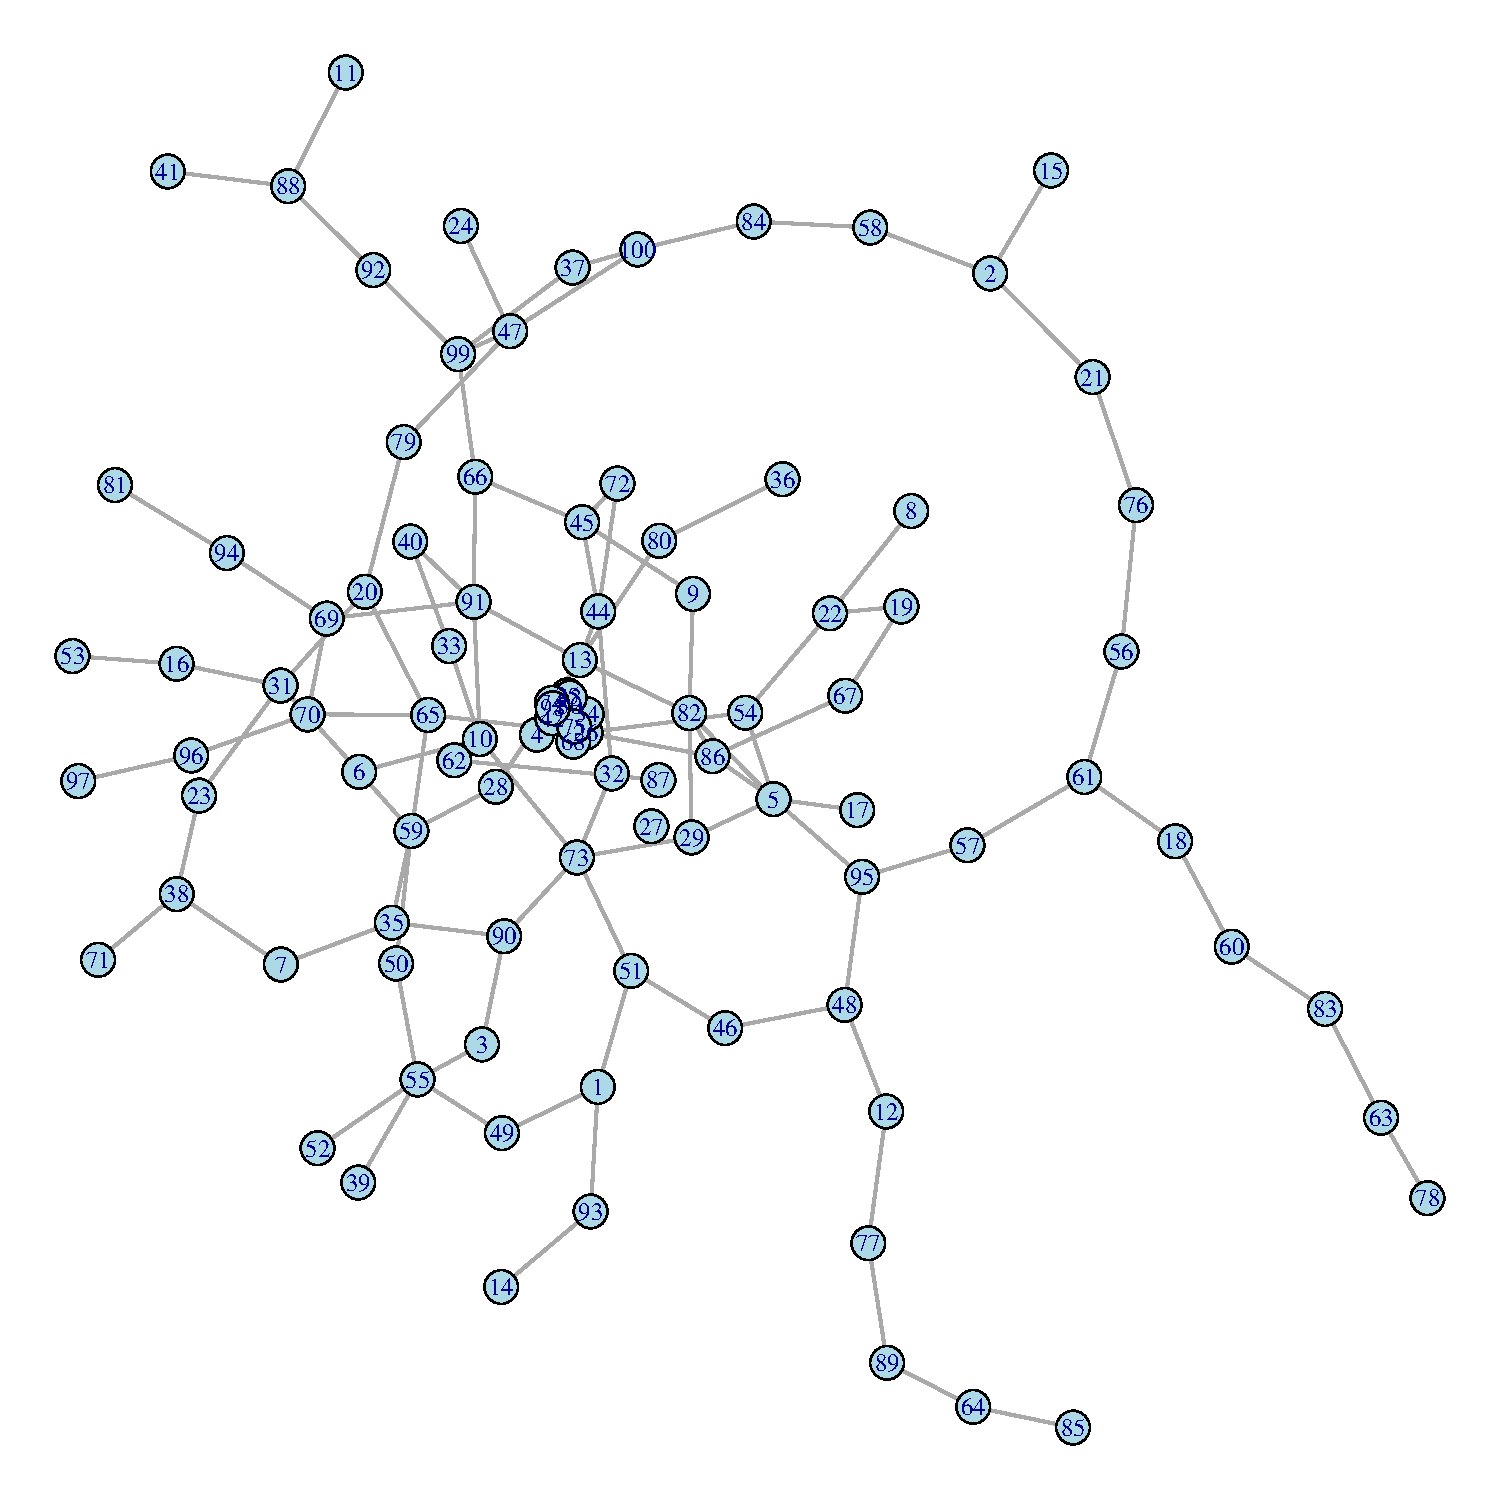
\includegraphics[height=0.85\textheight]{kamada}
 
\end{frame}

%------------------------------------------------

\begin{frame}
\frametitle{\insertsection}
\framesubtitle{Layout: Fruchterman and Reingold}

{\color{blue}{\cite{Fruchterman1991}}}
    \begin{itemize}
    \item Nodes as ``{\color{blue}{atomic particles or celestial bodies}} exerting attractive and repulsive forces from one another''
    \item {\color{blue}{Attractive forces}}: proportional to the square of the shortest distance between two nodes
    \item {\color{blue}{Repulsive forces}}: inversely proportional to the shortest distance between two nodes
    \end{itemize}

\end{frame}

%------------------------------------------------

\begin{frame}
\frametitle{\insertsection}
\framesubtitle{Layout: Fruchterman and Reingold}

\centering
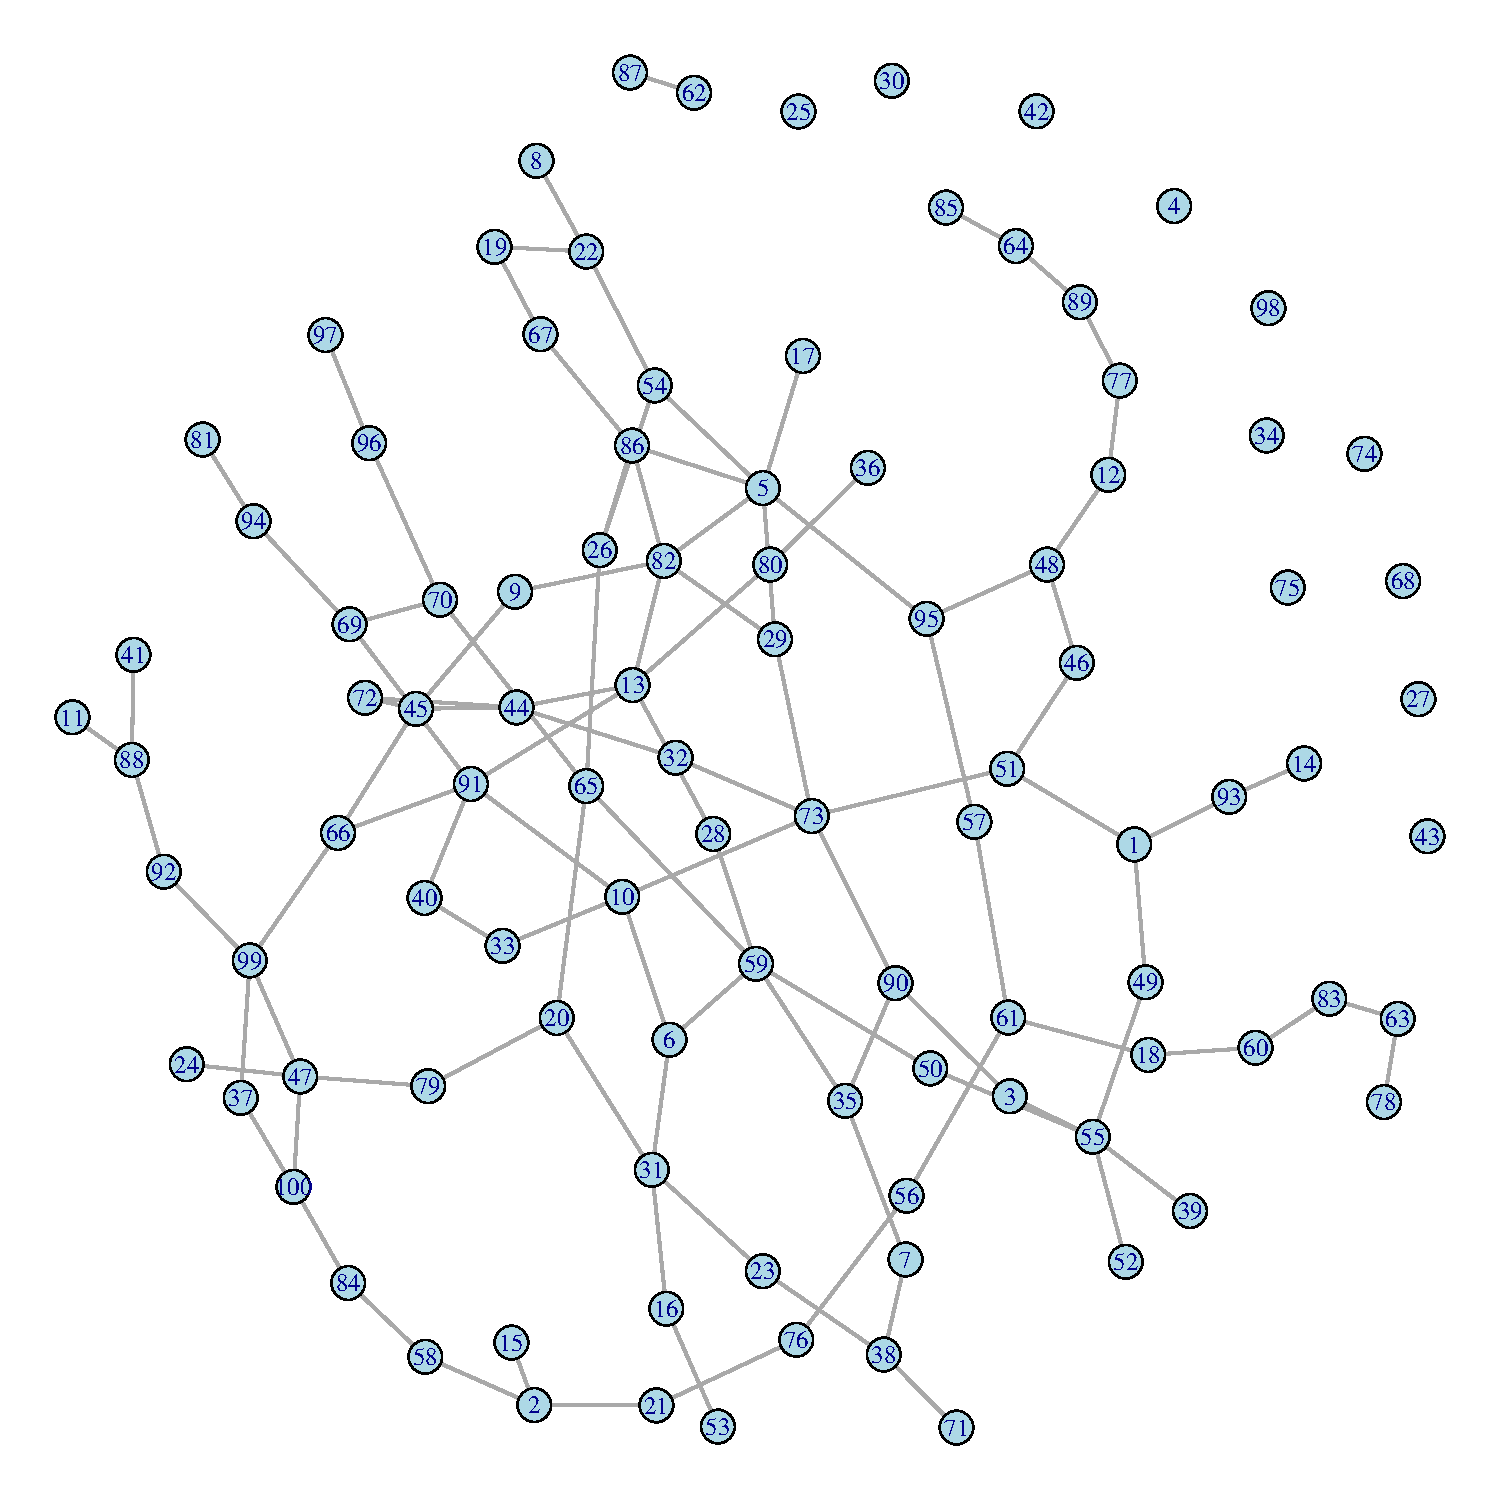
\includegraphics[height=0.85\textheight]{fr}
 
\end{frame}

%------------------------------------------------

\begin{frame}
\frametitle{\insertsection}
\framesubtitle{Layout: Kamada-Kawau and Fruchterman and Reingold in igraph}

\begin{columns}
\column{.5\textwidth}
\centering
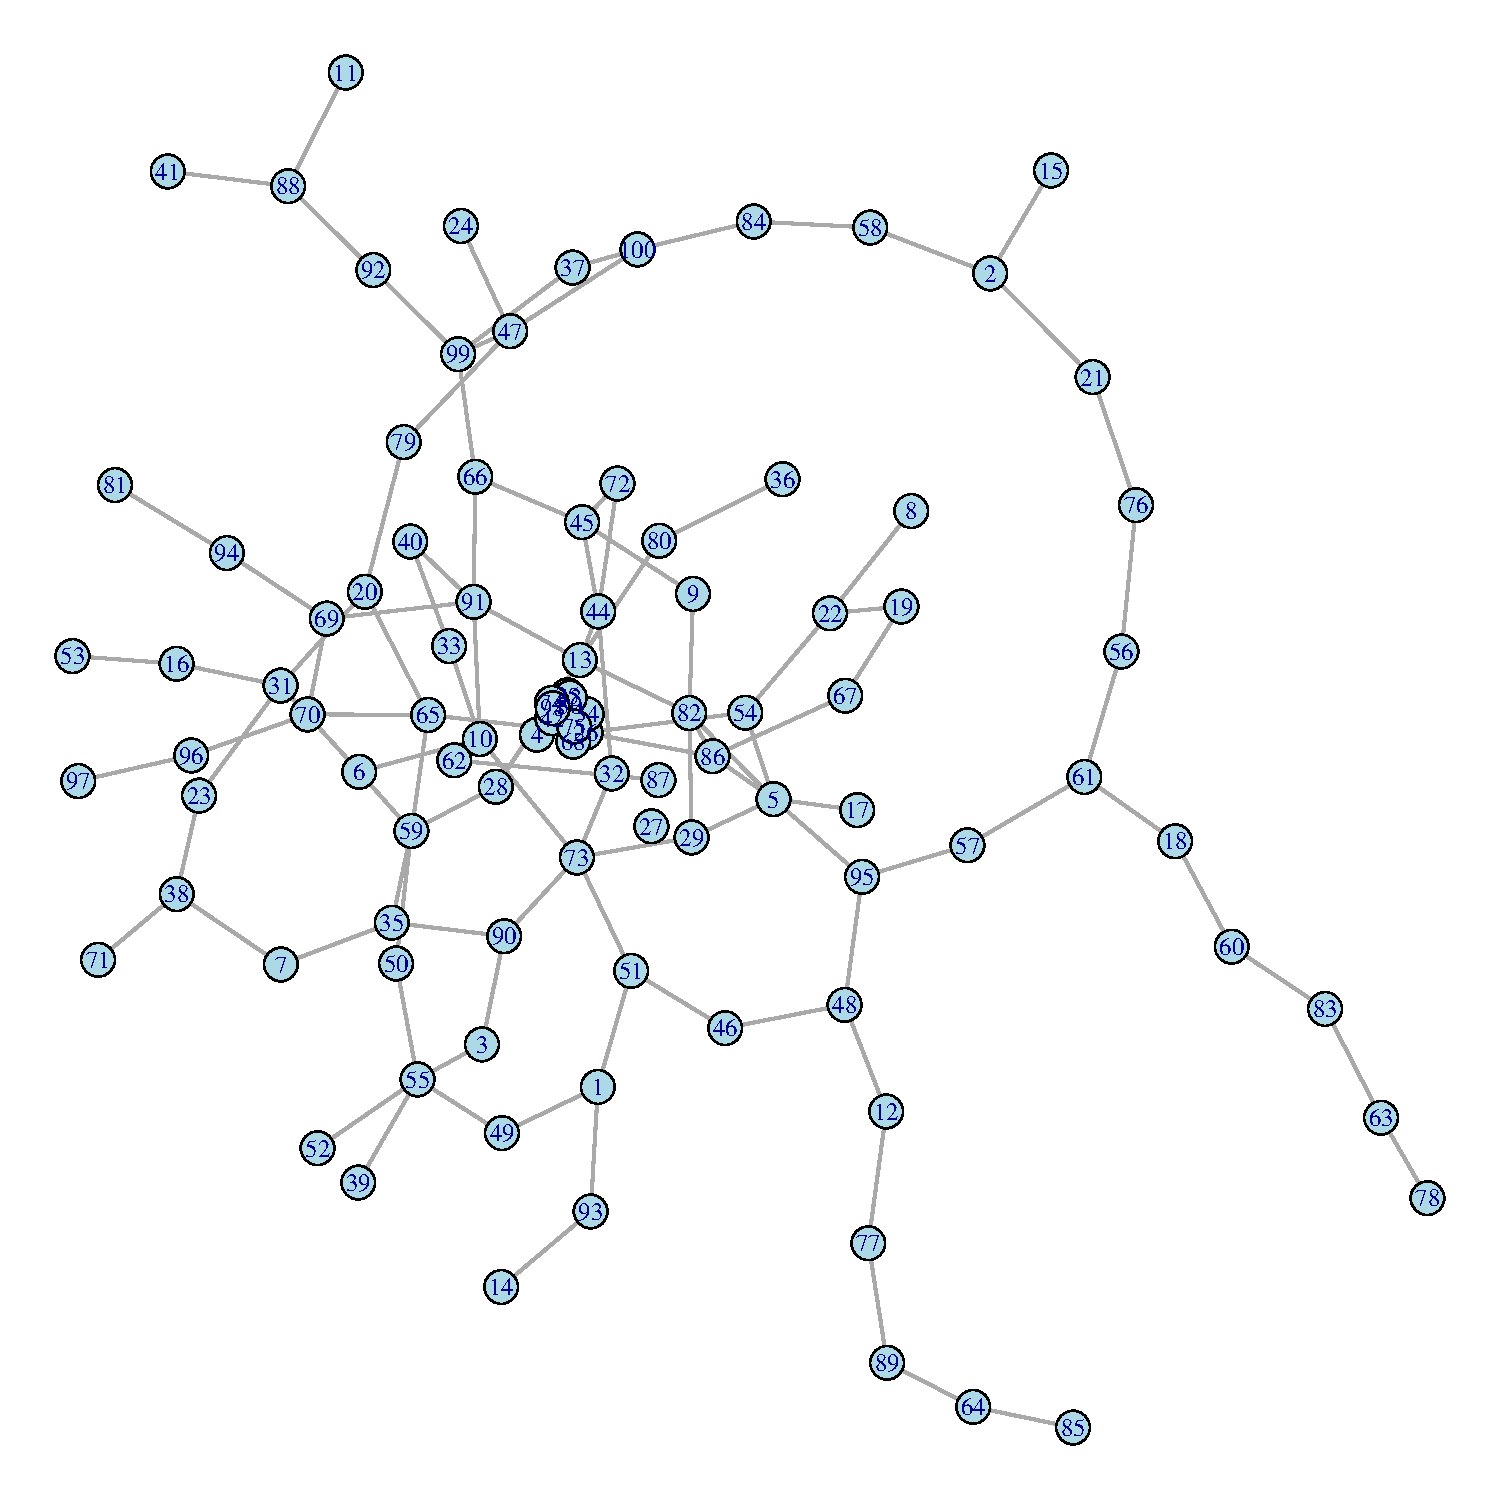
\includegraphics[width=0.4\linewidth]{kamada}\\
\lstinputlisting[language=R, firstline=43, lastline=47]{handouts_script/L7_script_handouts.R}

\column{.5\textwidth}
\centering
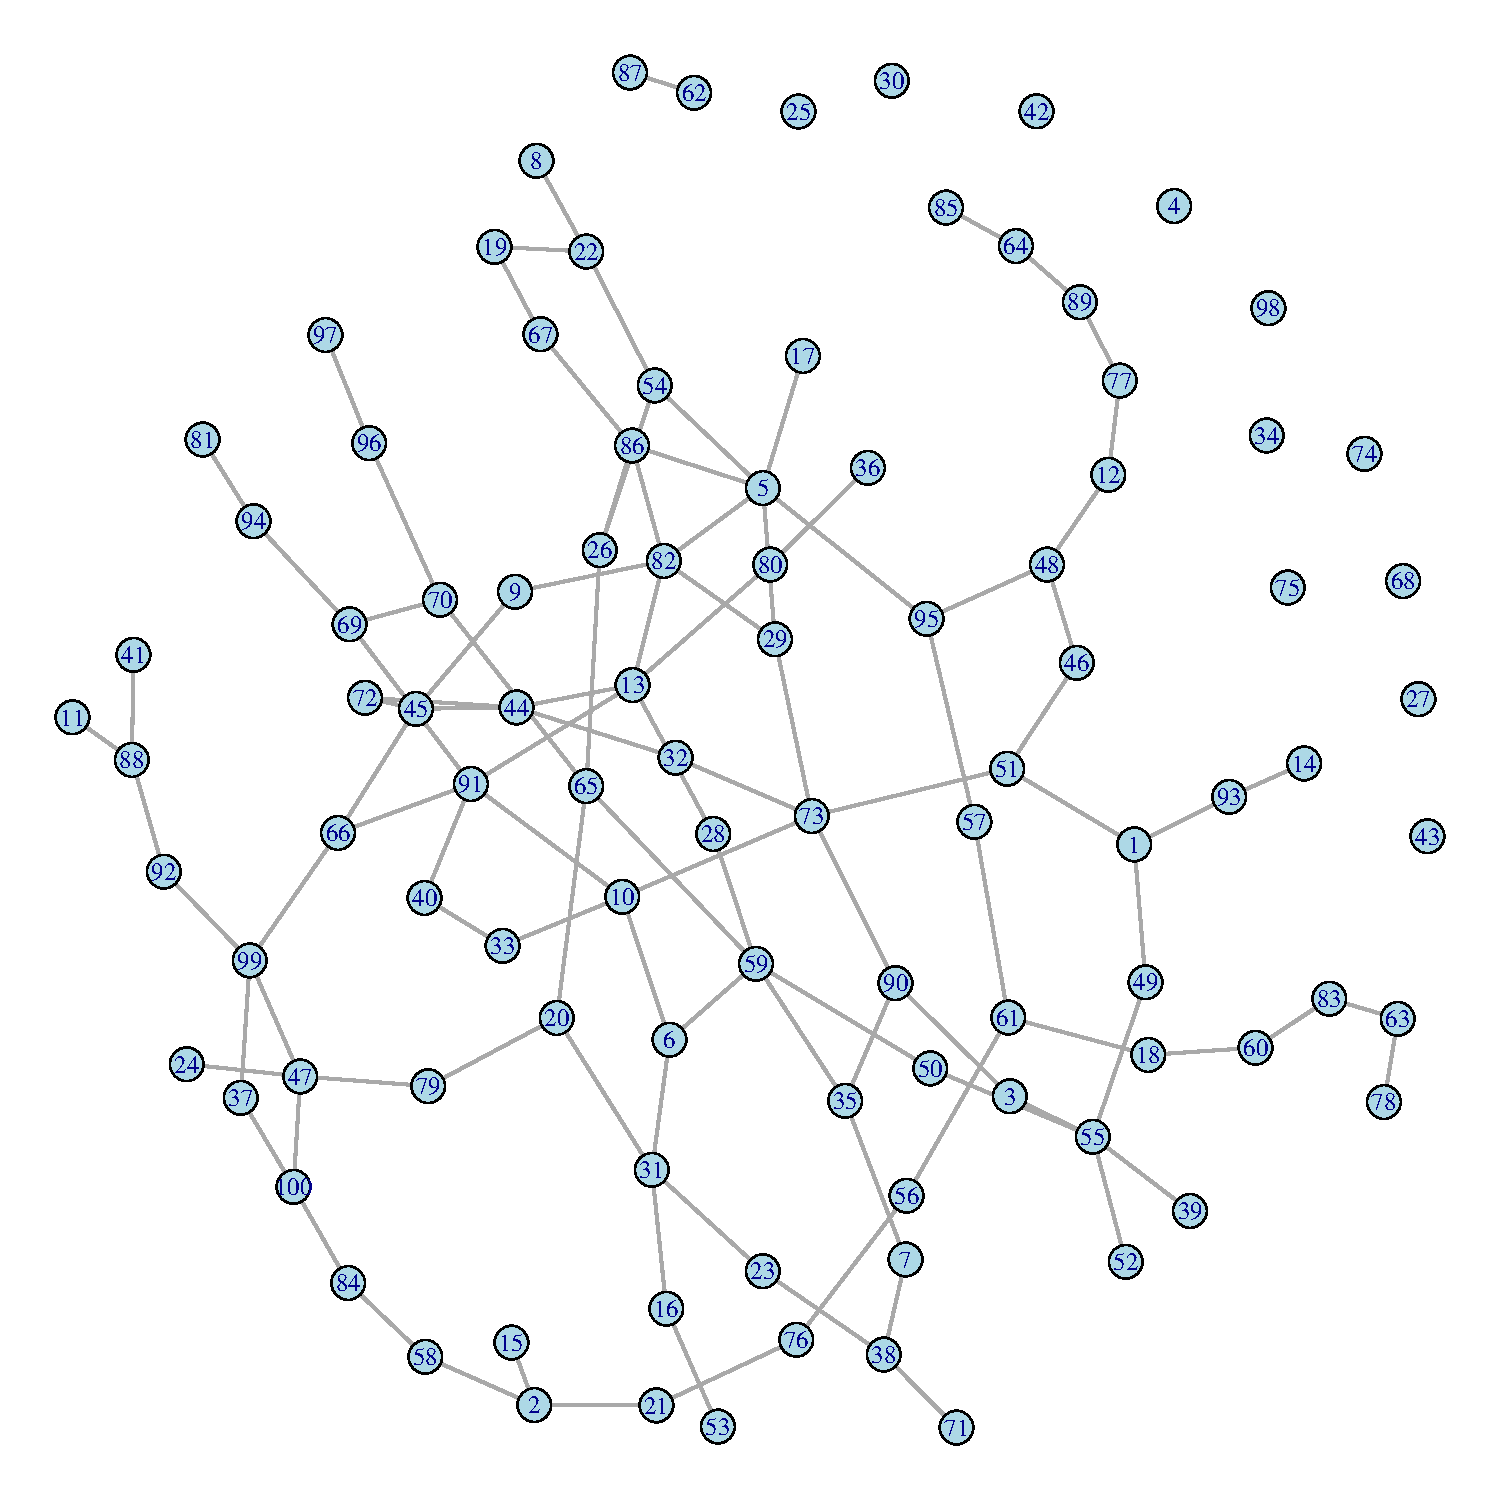
\includegraphics[width=0.4\linewidth]{fr}\\
\lstinputlisting[language=R, firstline=51, lastline=55]{handouts_script/L7_script_handouts.R}

\end{columns}

\end{frame}

%------------------------------------------------









%=======================================================
%	Questions
%=======================================================
\bgroup
\setbeamercolor{background canvas}{bg = orange}
\begin{frame}[plain]{}
\begin{center}
\color{white}{\Huge Questions}
\end{center}
\end{frame}
\egroup





%%=======================================================
%	Next time ...
%%=======================================================
\section*{Next time ...}

%------------------------------------------------

\bgroup
\setbeamercolor{background canvas}{bg = navyblue}
\begin{frame}[plain]{}
\begin{center}
\color{white}{\Huge\insertsection}
\end{center}
\end{frame}
\egroup

%------------------------------------------------

\begin{frame}
\frametitle{\insertsection}

\begin{itemize}

\item 	\textbf{Seminar: Principles of infographics}
	\begin{itemize}
	\item Network layout algorithms in igraph
	\item Import data in Gephi
	\item Visualise and analyse networks in Gephi
	\end{itemize}
	

\medskip
\medskip

\item 	\textbf{Lecture: Network models}
	\begin{itemize}
	\item Mathematical models of network analysis
	\item Overview of statistical models of network analysis
	\end{itemize}	
		
\end{itemize}

\end{frame}

%------------------------------------------------






%=======================================================
%	References
%=======================================================
\begin{frame}[allowframebreaks]
\frametitle{References}
\tiny
\bibliographystyle{apalike}
\bibliography{/Users/dr213/Dropbox/References/bibtex_references/library.bib}
\end{frame}
%------------------------------------------------






\end{document}